% ---------------------------------------------------------------------------
% Chapter 7: The Family Photograph: Generator-Level Jets and Truth Definitions
% The scripts, records and figures discussed here live in example/GenJet/ of
% https://github.com/ravindkv/JitJet . The book gives the physics and the
% instructions; the code itself is read on GitHub, not printed here.
% ---------------------------------------------------------------------------
%% chapter-local shorthands
\providecommand{\Bbar}{\ensuremath{\bar B^0}\xspace}
\providecommand{\Bz}{\ensuremath{B^0}\xspace}
\providecommand{\Lbbar}{\ensuremath{\bar\Lambda_b^0}\xspace}
\providecommand{\akfour}{\code{ak4GenJets}\xspace}
\providecommand{\akfournonu}{\code{ak4GenJetsNoNu}\xspace}
\providecommand{\akeight}{\code{ak8GenJets}\xspace}
\providecommand{\hadflav}{\code{hadronFlavour}\xspace}
\providecommand{\partflav}{\code{partonFlavour}\xspace}
\providecommand{\dij}{\ensuremath{d_{ij}}\xspace}
\providecommand{\diB}{\ensuremath{d_{iB}}\xspace}
\providecommand{\uik}{\ensuremath{u_{ik}}\xspace}
\chapter{The Family Photograph: Generator-Level Jets and Truth Definitions}
\chaptermark{The Family Photograph}
\label{ch:family_photograph}

\begin{journeybox}
Before the family leaves we take a photograph. Everyone who later claims to be a
member will be compared against it. But even a photograph involves choices: do
we include the neutrinos, and who decides whether this is a $b$ family at all?
\end{journeybox}

\physicsline{the generator-level jet as the reference of every later
chapter, the anti-$k_T$ distance and why the hard core comes first, the
three choices of radius, neutrinos and threshold, ghost association and
the hadron and parton flavour labels of \CMSSW, the physics and the
$\Delta R$ definitions and where they fail, the net flavour and its
infrared problem, flavour-$k_T$ and interleaved flavour neutralisation,
the reference GenJet of our $b$ jet}

\section{Welcome back: what we will see at this sixth stop}
\label{sec:family_photograph:what_we_compute}

At the end of \cref{ch:children_producing_grandchildren} the record held
749 particles that the detector will see, and the mother's family, the
descendants of the \Bbar ($b\bar d$), was a cluster of fifteen of them
around $\eta=-1.4$, $\phi=-2.7$, inside a cone of $\dR<0.4$ around the
quark that held $99.43\GeV$. Nothing happens to the particles at this
stop. What happens is a decision: before the family walks into the
detector of \cref{ch:crossing_the_border}, where it will be smeared,
split, merged with the crowd of \cref{ch:crowd_on_the_road} and
reassembled from tracks and calorimeter cells, we take its photograph,
the \emph{generator-level jet}, and every reconstructed jet of
\crefrange{ch:the_inn}{ch:registry_office_top} will be judged by how well it
reproduces that photograph. The cone around the quark was our own
bookkeeping; the photograph is taken by the algorithm the experiment
uses, \antikt with $R=0.4$ run on the stable particles, exactly as the
\code{GenJet} producers of \CMSSW run it, and it is the reference of the
jet energy corrections of \crefrange{ch:paying_for_uninvited}{ch:the_receipt}
and of every flavour efficiency of \cref{ch:footprints}. This stop builds
that photograph by hand: the sequential recombination with its distance,
the three choices that change the picture without changing the family,
and then the question the journey box asks, who decides that the jet is
a $b$ jet. The experiment's answer is a ghost: the B~hadron, which has
decayed and is no longer in the picture, is put back with its direction
and a momentum of $10^{-18}$ of its own, and the jet that catches the
ghost is the $b$ jet. The theorist's answer is harder, because a label
that a soft gluon splitting into a $b\bar b$ pair can change is not a
quantity that a perturbative calculation can predict, and the last part
of the chapter follows the two repairs of the literature, flavour-$k_T$
and interleaved flavour neutralisation, far enough to run them on our
event.

The numbers to take away are three. The \antikt jet of $R=0.4$ around the
mother holds $99.83\GeV$ in 31 particles, $0.4$ more than the cone,
because its axis is free to follow the family; the jet without the
neutrinos is the same jet in our event, and $8\GeV$ poorer on average over
four hundred decays; the jet of $R=0.8$ holds $105.79$. The ghost of the
\Bbar lands in that jet in every one of four hundred decays, so that the
label is never in doubt for this family; the hard-process $b$ quark,
however, points $0.56$ away from the jet, outside it, because the initial
state radiation of \cref{ch:mother_gives_birth} gave the hard system a
recoil, and a definition that asks the hard-process parton finds nothing.
And a $b\bar b$ pair of half a GeV, placed between two light jets, changes
both their labels under the experiment's definition and leaves them
unchanged under the safe ones. As at the previous stops we meet the
numbers four times, from the top down:
\begin{enumerate}[nosep]
  \item \textbf{Watch it.} A film shows the 749 particles becoming 42 jets,
    the \antikt algorithm building our jet merge by merge from the hard
    core outward, the radius growing and the neutrino leaving, the
    B~hadron shrinking to a ghost and still landing in the jet, a soft
    $b\bar b$ pair relabelling two jets and being neutralised, and the
    same family photographed four hundred times
    (\cref{sec:family_photograph:animation}).
  \item \textbf{Run it.} A Python file, needing only NumPy, clusters the
    record of \cref{ch:children_producing_grandchildren} into the three
    \CMSSW collections, assigns every label and writes the jet tables, in
    fifteen seconds (\cref{sec:family_photograph:standalone_code}).
  \item \textbf{Derive it.} Why the hard particle sets the distance and the
    jet is built from the inside out, what the radius, the neutrinos and
    the threshold do, how a ghost follows the clustering without moving it
    and what \hadflav and \partflav mean, why the physics definition fails
    in our event, why the net flavour is not infrared safe and how the two
    safe definitions repair it
    (\crefrange{sec:family_photograph:what_we_mean_by_the_true_jet_choices_and}{sec:family_photograph:infrared_safe_flavour_flavour_k_t_and_in}).
  \item \textbf{Check it against the official packages.} \FASTJET, the
    library every experiment calls, and \PYTHIA's own \code{SlowJet}
    cluster exactly our 749 particles and reproduce every jet, every
    constituent list and every label; \FASTJET runs on two thousand events
    of \PYTHIA's full chain; and the CMS generator job of
    \cref{ch:ancestral_home} drew its sixth, seventh and eighth figures at
    this stage (\cref{sec:family_photograph:validation}).
\end{enumerate}

\Cref{tab:family_photograph:numbers} gives away the ending. The sharpest
column pair is, once more, a comparison on identical input: the 749
particles of \file{event_Decay.lhe} clustered by \FASTJET~3.5.2 and by the
script, with the same ghosts. They agree exactly, to the last digit of
every jet momentum and to the last constituent, which is what a port of a
deterministic algorithm must do; the interesting columns are the ones
that vary, the four hundred decays of the same hadrons clustered each
time, \PYTHIA's full chain with \FASTJET, and the \CMSSW event.

\begin{table}[htbp]\centering\small
\caption[Generator-level jets obtained four ways]{Generator-level jets
obtained four ways. ``Same particles'' means the 749 final particles of
\file{example/Decay/event_Decay.lhe} with the same ghosts, clustered by
\FASTJET~3.5.2 and by the standalone script; ``400 decays'' means the
primary hadrons of \cref{ch:children_getting_married} decayed four hundred
times with the script of \cref{ch:children_producing_grandchildren} and
clustered each time; ``full chain'' means \PYTHIA from the hard event of
\cref{ch:ancestral_home} with the CP5 settings, $2000$ events, clustered
with \FASTJET and the same ghosts, the status-71 copy of the quark as the
axis. The spread of a single event follows $\pm$. ``Response'' is
$\pt(\mathrm{jet})/\pt(b)$ with the last copy of the quark before the
hadronisation, which in the full chain fluctuates itself. The \CMSSW
column is the single event of \cref{ch:ancestral_home}, read from pages
6 to 8 of its analyser's output.}
\label{tab:family_photograph:numbers}
\scriptsize\setlength{\tabcolsep}{3pt}
\resizebox{\textwidth}{!}{%
\begin{tabular}{lrrrrr}\toprule
 & \FASTJET & standalone & standalone & \PYTHIA + \FASTJET & \CMSSW \\
 & same particles & same particles & 400 decays & full chain & 1 event \\ \midrule
\akfour: jets above $3$ / $10$ / $30\GeV$ & $42$ / $11$ / $6$ & $42$ / $11$ / $6$ & $40.0\pm2.2$ / $10.2$ / $6.0$ & $18.2\pm11.5$ / $3.9$ / $2.4$ & $27$ / -- / -- \\
\quad particles clustered, of & $368$ of $749$ & $368$ of $749$ & $357\pm16$ & $152\pm88$ & $239$ of $634$ \\
\akeight: jets, particles clustered & $30$, $600$ & $30$, $600$ & $30.4$, $608$ & $20.2$, $321$ & $28$, $488$ \\ \midrule
$b$ quark (last copy): \pt [GeV] & $78.29$ & $78.29$ & $78.29$ & $95.5\pm30.0$ & $91.74$ \\
$b$ jet, \akfour: \pt [GeV], $n$ & $99.830$, $31$ & $99.830$, $31$ & $99.63\pm0.49$, $25.7$ & $109.9\pm27.6$, $21.3$ & $117.79$, $24$ \\
\quad response, \dR to the quark & $1.275$, $0.062$ & $1.275$, $0.062$ & $1.273\pm0.006$, $0.060$ & $1.22\pm0.51$, $0.028$ & $1.284$, $0.019$ \\
\quad the cone of the same $R$ [GeV] & $99.43$ & $99.43$ & $98.79\pm0.68$ & $109.7\pm26.5$ & -- \\
\quad neutrino \pt inside [GeV] & $0$ & $0$ & $7.7$ (none in $54\%$) & $7.9$ (none in $58\%$) & $37.5$ \\
$b$ jet, \akfournonu: \pt [GeV] & $99.830$ & $99.830$ & $91.93\pm12.12$ & $102.1\pm28.9$ & $79.82$ \\
$b$ jet, \akeight: \pt [GeV], $n$ & $105.786$, $47$ & $105.786$, $47$ & $104.61\pm0.80$, $41.3$ & $120.0\pm24.6$, $34.3$ & $141.10$, $55$ \\
$b$ jet: \hadflav $=5$, $|\partflav|=5$ [\%] & $5$, $5$ & $5$, $5$ & $100$, $100$ & $99.2$, $99.3$ & -- \\
$b$ jet: physics flavour, $\dR<0.3$ flavour & $0$, $+5$ & $0$, $+5$ & -- & -- & -- \\
$b$ jet: net $b$ flavour $+1$ / $-1$ [\%] & $+1$ & $+1$ & $83.2$ / $16.8$ & -- & -- \\
$b$ jet: B hadron to the axis, its products outside & $0.06$, $0$ & $0.06$, $0$ & $0.062$, $0.20$ & $0.025$, $0.31$ & -- \\ \midrule
$\bar b$ jet, \akfour: \pt [GeV], response & $94.093$, $1.298$ & $94.093$, $1.298$ & $93.86\pm0.83$, $1.295$ & $106.5\pm20.9$, $1.23$ & $115.94$, $0.996$ \\
$\bar b$ jet, \akeight: \pt [GeV], \dR & $147.688$, $0.361$ & $147.688$, $0.361$ & $113.4\pm20.4$, $0.14$ & $115.3\pm17.0$, $0.05$ & $121.01$, $0.022$ \\
$\bar b$ jet: net $b$ flavour $-1$ / $+1$ [\%] & $+1$ (oscillated) & $+1$ (oscillated) & $79.2$ / $20.8$ & -- & -- \\
\akfour jets with two $b$ hadrons per event & $1$ & $1$ & $1.00$ & $0.009$ & -- \\
IFN neutralisations per event & $0$ & $0$ & $0.66$ & -- & -- \\
\bottomrule
\end{tabular}}
\end{table}

\begin{figure}[htbp]\centering
\resizebox{\textwidth}{!}{% ---------------------------------------------------------------------------
% The family photograph: (a) the b family of our event at stage 5 (the final
% particles of the Bbar0 and the neighbours within the cone) with the three
% photographs anti-kT takes of it, R = 0.4 with and without the neutrino and
% R = 0.8; (b) the three choices that change the picture but not the family.
% Numbers: event_GenJet.lhe (seed 1), the ensemble of 400 decays, and the
% CMSSW event (pages 6-8 of genJetAnalyzer_ME_PS_MPI_Had_Decay_GenJet_out.pdf).
% ---------------------------------------------------------------------------
\begin{tikzpicture}[x=1cm,y=1cm,
  every node/.style={font=\footnotesize},
  lab/.style={font=\scriptsize,align=center},
  head/.style={font=\small\bfseries},
  fam/.style={circle,fill=red!75!black,inner sep=0pt},
  oth/.style={circle,fill=black!40,inner sep=0pt},
  nu/.style={circle,draw=green!50!black,thick,fill=white,inner sep=0pt},
  ring4/.style={red!80!black,line width=1.6pt},
  ring8/.style={blue!70!black,line width=1.2pt,dashed},
  box/.style={draw,rounded corners=3pt,thin,fill=gray!6,align=left,inner sep=5pt,text width=5.0cm,font=\scriptsize}]
% ---------------- (a) the family and its photographs --------------------------------------------
\begin{scope}
\node[head,anchor=west] at (-4.4,4.6) {(a) the $b$ family at stage 5 and the photographs anti-$k_T$ takes of it};
% the (eta, phi) frame, 1 unit = 3 cm
\draw[-{Stealth}] (-4.0,-3.6) -- (4.0,-3.6) node[below left,lab] {$\eta$};
\draw[-{Stealth}] (-4.0,-3.6) -- (-4.0,3.9) node[left,lab] {$\phi$};
\foreach \x in {-3,-1.5,0,1.5,3} {\draw (\x,-3.65) -- (\x,-3.55);}
\foreach \y in {-3,-1.5,0,1.5,3} {\draw (-4.05,\y) -- (-3.95,\y);}
\node[lab,anchor=north] at (0,-3.7) {$0.5$ units of $\Delta R$ per tick};
% the rings
\draw[ring8] (0,0) circle (2.4);
\draw[ring4] (0,0) circle (1.2);
\node[lab,text=red!80!black,anchor=south west] at (0.85,0.85) {$R=0.4$: $99.83\,\mathrm{GeV}$, 31 particles};
\node[lab,text=blue!70!black,anchor=south west] at (1.7,1.75) {$R=0.8$: $105.79\,\mathrm{GeV}$, 47};
% the family: the Bbar0's 15 final descendants (red), the core very close
\foreach \p/\s in {(0.05,0.1)/5.5,(-0.1,-0.05)/4.5,(0.15,-0.15)/4.0,(-0.2,0.2)/3.2,(0.3,0.05)/3.0,(-0.05,0.35)/2.6,(0.25,-0.35)/2.4,(-0.4,-0.2)/2.2,(0.45,0.3)/2.0,(-0.35,0.5)/1.8,(0.55,-0.1)/1.6,(0.1,-0.6)/1.5,(-0.6,0.1)/1.4,(0.7,0.5)/1.3,(-0.5,-0.6)/1.2} {\node[fam,minimum size=\s pt] at \p {};}
% the neighbours inside R = 0.4 (grey), the periphery
\foreach \p/\s in {(0.9,0.6)/2.0,(-0.95,0.4)/1.8,(0.6,-0.9)/1.6,(-0.7,-0.8)/1.5,(1.05,-0.2)/1.4,(-0.3,1.0)/1.3,(0.2,1.1)/1.2,(-1.1,-0.1)/1.2,(0.95,-0.65)/1.1,(-0.8,0.85)/1.1,(0.4,-1.1)/1.0,(-0.15,-1.05)/1.0,(1.1,0.3)/1.0,(-1.0,-0.55)/1.0,(0.75,1.0)/0.9,(-0.55,1.05)/0.9} {\node[oth,minimum size=\s pt] at \p {};}
% between 0.4 and 0.8: the gluon's family and more soft stuff
\foreach \p/\s in {(1.6,0.9)/2.6,(1.9,0.5)/2.0,(1.5,1.4)/1.6,(2.1,1.1)/1.4,(-1.7,-1.2)/1.3,(-1.9,0.6)/1.2,(0.5,-2.0)/1.2,(-0.4,2.1)/1.1,(2.2,-0.7)/1.1,(-2.1,-0.4)/1.0,(1.2,-1.8)/1.0,(-1.3,1.7)/1.0,(0.9,2.1)/0.9,(-2.0,1.3)/0.9,(1.8,-1.4)/0.9,(-0.9,-2.1)/0.9} {\node[oth,minimum size=\s pt] at \p {};}
% outside
\foreach \p/\s in {(3.2,1.5)/1.4,(-3.1,-2.4)/1.2,(2.9,-2.6)/1.3,(-2.9,2.6)/1.1,(3.4,-0.6)/1.0,(-3.4,0.9)/1.0,(1.0,3.2)/1.0,(-1.4,-3.1)/1.0,(3.1,3.0)/0.9,(-3.3,-1.0)/0.9} {\node[oth,minimum size=\s pt] at \p {};}
% the quark and the axis
\node[star,star points=5,draw=black,fill=white,inner sep=1.4pt] at (-0.17,-0.06) {};
\node[lab,anchor=north east] at (-0.2,-0.2) {$b$ quark, $78.3$};
\node[star,star points=5,fill=red!80!black,inner sep=1.3pt] at (0,0) {};
% the neutrino of the semileptonic decay (seed 4), hollow
\node[nu,minimum size=6pt] at (-0.3,-0.4) {};
\node[lab,text=green!50!black,anchor=north east,align=right] at (-0.4,-0.5) {$\nu$ of decay seed 4:\\ $9.4\,\mathrm{GeV}$, in the ring,\\ not in the detector};
\node[lab,anchor=south west,text width=4.1cm,align=left,text=black!65] at (-4.0,-3.4) {red: the $\bar B^0$'s descendants, $78.3\,\mathrm{GeV}$;\\ grey: the rest of the event; the axis (red star) is the jet's, $0.06$ from the quark};
\end{scope}
% ---------------- (b) the choices ------------------------------------------------------------------
\begin{scope}[xshift=10.2cm]
\node[head,anchor=west] at (-0.6,4.6) {(b) three choices change the picture, not the family};
\node[box,anchor=north west] (C1) at (-0.6,3.9) {\textbf{the radius $R$}\\ $0.4$: $99.83\,\mathrm{GeV}$ (ak4GenJets)\\ $0.8$: $105.79\,\mathrm{GeV}$ (ak8GenJets)\\ the cone around the quark: $99.43$ and $108.73$\\ beyond $R\simeq1$ the neighbouring gluon jet is swallowed};
\node[box,anchor=north west,below=4mm of C1.south west] (C2) {\textbf{the neutrinos}\\ ak4GenJets keeps them, ak4GenJetsNoNu does not\\ our event: the same jet ($99.83$), no neutrino\\ decay seed 4 of the same hadrons: $99.6\to90.2$\\ 400 decays: $99.63\pm0.49\to91.93\pm12.12$\\ CMSSW's event: $117.8\to79.8$ ($37.5\,\mathrm{GeV}$ of $\nu$)};
\node[box,anchor=north west,below=4mm of C2.south west] (C3) {\textbf{the threshold}\\ jets above $3\,\mathrm{GeV}$ (GenJet): 42\\ above $10$: 11; above $30$: 6\\ CMSSW's event: 27 jets above $3\,\mathrm{GeV}$};
\node[lab,anchor=north west,text width=5.2cm,align=left,text=black!65,below=4mm of C3.south west] {Every later chapter compares a reconstructed jet with one of these photographs and must say which: CMS calibrates to the one without neutrinos.};
\end{scope}
\end{tikzpicture}
}
\caption[The family photograph: the $b$ family and the pictures anti-$k_T$
takes of it]{The family photograph. Left: the $b$ family of our event at
stage~5, the fifteen descendants of the \Bbar ($b\bar d$) in red and the
rest of the event in grey around the jet axis, with the two circles that
\antikt draws, $R=0.4$ and $0.8$, and the neutrino of decay seed~4 of the
ensemble, which sits inside the ring and outside the detector. Right: the
three choices that change the picture but not the family, with the
numbers of our event, of four hundred decays and of the \CMSSW event.}
\label{fig:family_photograph:photograph_sketch}
\end{figure}

\paragraph{A picture to carry: the photograph.} The family of
\cref{fig:family_photograph:photograph_sketch} is what the decays left:
fifteen particles from the \Bbar within a tenth of a unit of each other,
sixteen more from the gluons and the underlying event within $0.4$, and a
scatter of soft particles everywhere. The photograph is a rule for
drawing a circle around them. \antikt draws it from the inside out, the
hardest particle first and everything within $R$ of it next, so that the
circle is round and centred on the hard core, and a soft particle at the
edge belongs or does not belong by its distance to that core alone. Two
things in the picture matter for everything that follows. The circle is
a choice three times over: its radius, $0.4$ for the small jets of this
book and $0.8$ for the boosted ones of \cref{ch:three_families}; whether
the neutrino inside it is counted, which CMS does not, because the
detector will not see it and a calibration against a photograph with
neutrinos would ask the detector to measure what it cannot; and the
threshold below which a circle is not a jet at all, $3\GeV$ for the
generator and $30$ or more for an analysis. And the label on the picture,
``$b$ jet'', is a second rule, laid on top of the first, which the
experiment answers with the B~hadron's ghost and the theory with a
definition that a soft gluon cannot change. The rules are the \antikt
paper~\cite{Cacciari:2008gp} and the \FASTJET manual~\cite{Cacciari:2011ma},
the \CMSSW producers \code{GenJetParticles}, \code{FastjetJetProducer}
and \code{JetFlavourClustering}, and, for the last section, the
flavour-$k_T$ of Banfi, Salam and Zanderighi~\cite{Banfi:2006hf} and the
interleaved flavour neutralisation of Caola, Grabarczyk, Hutt, Salam,
Scyboz and Thaler~\cite{Caletti:2022glq}. The algorithms themselves, their
history and the choice of $R$, are the business of \cref{ch:the_inn}; this
stop uses \antikt as the experiment's photographer and asks what the
photograph shows.

\section{Watch the photograph being taken: the animated journey}
\label{sec:family_photograph:animation}

The film first. \file{example/GenJet/Standalone/animate_standalone_genjets.py}
imports the standalone script of \cref{sec:family_photograph:standalone_code}
and clusters the seed-1 record in six narrated scenes of about five
minutes in all (eighty seconds without the voice), so that every number
on the screen and in the narration is produced by the classes that wrote
the jet tables. The voice picks up where the film of
\cref{ch:children_producing_grandchildren} stopped, the grandchildren are
born, and ends at the next stop, the crowd on the road of
\cref{ch:crowd_on_the_road}. It is on the JitJet playlist,
\begin{center}
  \url{https://www.youtube.com/playlist?list=PLbSW20iyZFd4}
\end{center}
and \cref{fig:family_photograph:stills} shows one key frame per scene.
Each scene names the section that explains it.
\begin{enumerate}
  \item \textbf{The photograph} (\cref{sec:family_photograph:our_jet_at_this_stage_the_reference_genj}).
    The 749 particles appear in the $(\eta,\phi)$ plane, hardest first,
    then the 42 circles of the \antikt jets settle over them, the leading
    eight in colour: the mother's family is jet [0] with $99.8\GeV$, the
    $\bar b$'s jet [1] with $94.1$.
  \item \textbf{Anti-$k_T$ gathers the family, hardest first} (\cref{sec:family_photograph:antikt}).
    Zoom on the $b$ jet: the 36 merges in their order, the $K^-$ and
    $\pi^-$ of the \Bbar at $\dR=0.006$ first, the photons, the ghosts
    slipping in, the soft periphery last at $\dR$ up to $0.38$, the
    running \pt and the ladder of distances, and the circle drawn when
    \diB wins.
  \item \textbf{The choices} (\cref{sec:family_photograph:choices}).
    The radius grows from $0.05$ to $0.9$ around the same axis and the \pt
    inside it with it, $99.8$ at $0.4$, $105.8$ at $0.8$; decay seed~4 of
    the same hadrons, in which the B went semileptonic, shows the jet
    without neutrinos at $90.2\GeV$ instead of $99.6$; the threshold
    counts $42$, $11$ and $6$ jets.
  \item \textbf{The ghosts} (\cref{sec:family_photograph:ghosts}).
    The \Bbar shrinks to a ghost of $10^{-18}$ of its momentum and still
    lands in jet [0]: \hadflav $5$; the $b$ quark's ghost gives \partflav
    $+5$; the status-23 quark sits outside. At the other end of the event
    the gluon's pair shares one jet and the oscillated \Bz gives the
    $\bar b$ jet a $b$.
  \item \textbf{The whisper} (\cref{sec:family_photograph:infrared_safe_flavour_flavour_k_t_and_in}).
    A $B^0\bar B^0$ pair of half a GeV appears between two light jets; the
    ghost and the net labels flip, the IFN distance cancels the pair, and
    the scan in the pair's \pt shows which definitions survive.
  \item \textbf{Again and again} (\cref{sec:family_photograph:our_jet_at_this_stage_the_reference_genj}).
    The same primary hadrons decayed and clustered four hundred times: the
    response of the \akfour, \akfournonu and \akeight jets to the quark
    fill their histograms, $1.273$, $1.174$ with a tail, $1.336$.
\end{enumerate}
Rendering needs matplotlib in addition to NumPy, \code{ffmpeg} for an
\code{.mp4}, and \code{edge-tts} for the voice (the shared
\file{example/soundtrack.py} synthesises the lines, caches the clips and
writes the score and the subtitles):
\begin{minted}[linenos=false,frame=single,framesep=1.5mm,fontsize=\small]{bash}
cd example/GenJet/Standalone
python3 animate_standalone_genjets.py            # the narrated film, 1080p, ~1 h with --jobs 4
python3 animate_standalone_genjets.py --fast     # low-resolution preview
python3 animate_standalone_genjets.py --print-script   # the narration, one line per phase
python3 animate_standalone_genjets.py --scene gather,ghosts -o g.gif   # silent
python3 animate_standalone_genjets.py --stills stills.pdf --no-video
\end{minted}
\code{--no-narration} gives the silent cut; the ensemble of scene~6 is read
from the statistics file of \cref{sec:family_photograph:standalone_code}
when it exists.

\begin{figure}[htbp]\centering
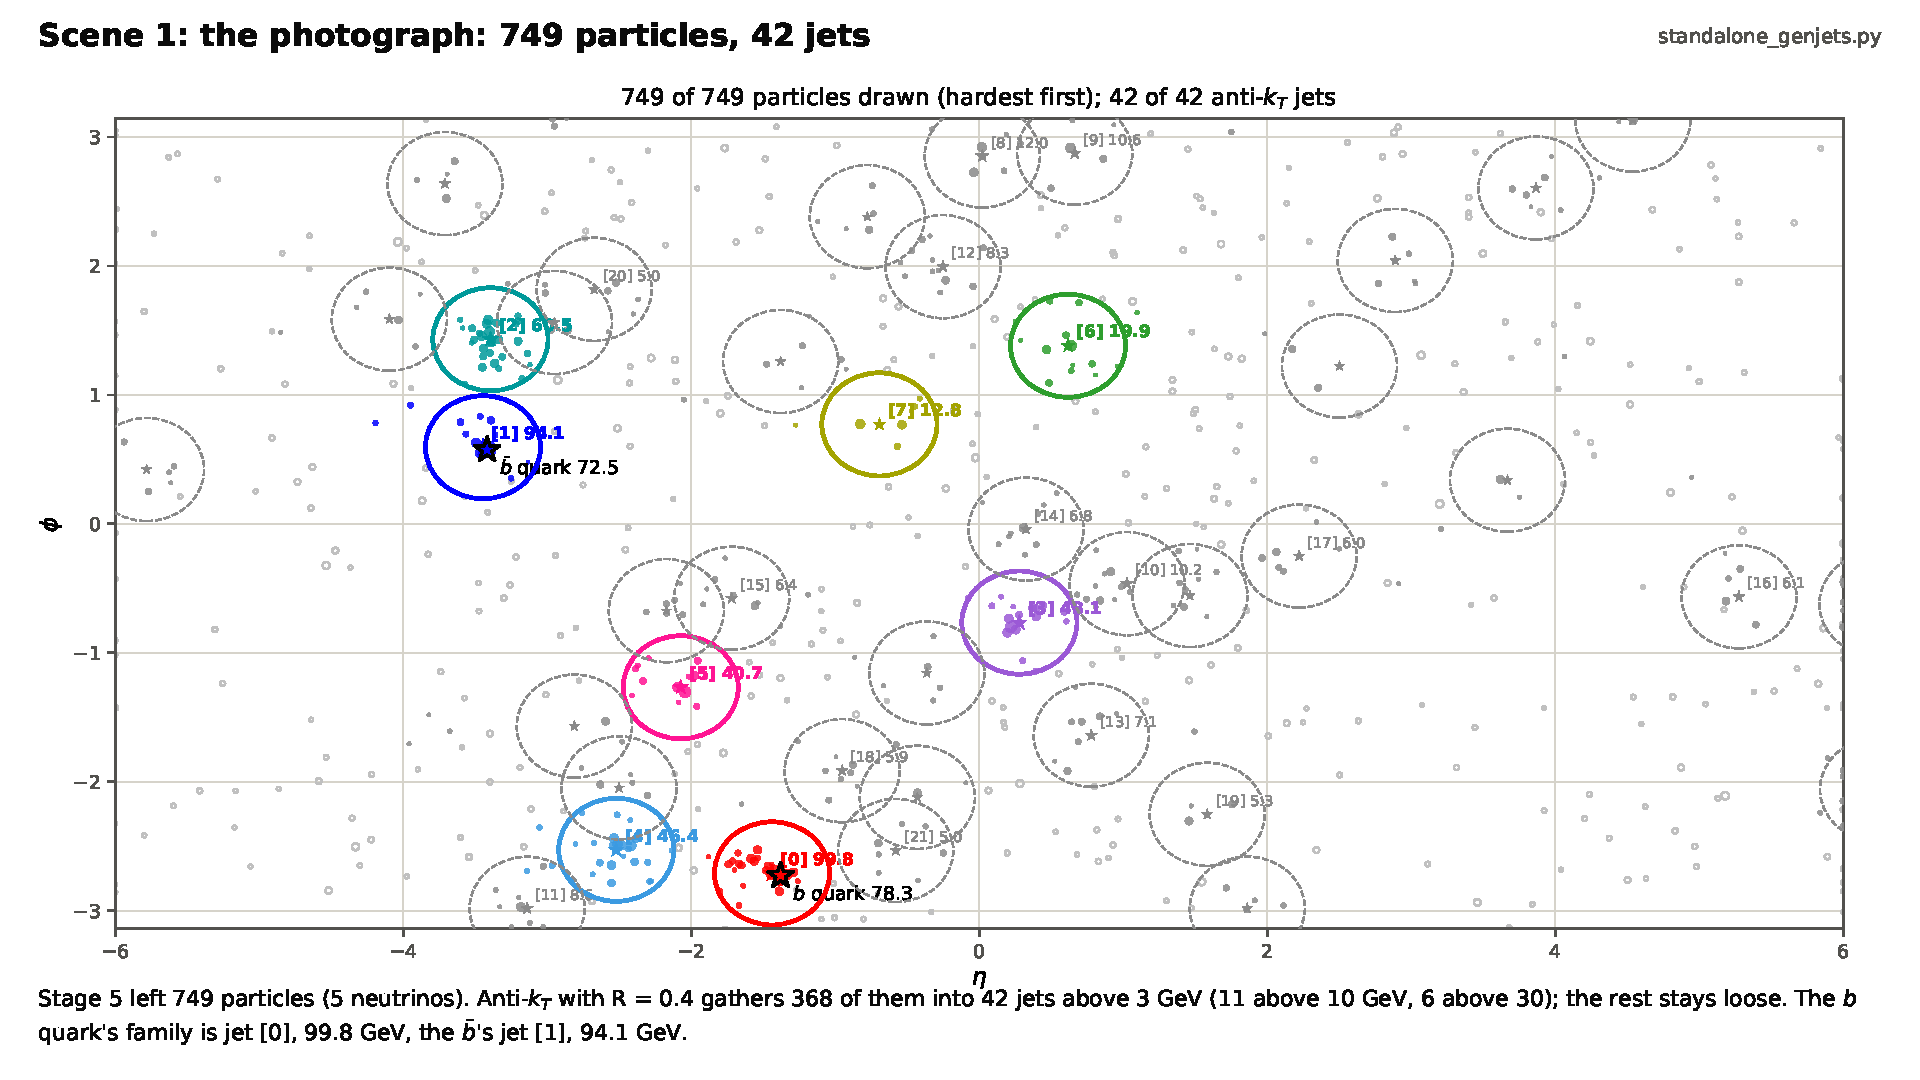
\includegraphics[page=1,width=0.325\textwidth]{GenJet/Standalone/animate_standalone_genjets_stills.pdf}\hfill
\includegraphics[page=2,width=0.325\textwidth]{GenJet/Standalone/animate_standalone_genjets_stills.pdf}\hfill
\includegraphics[page=3,width=0.325\textwidth]{GenJet/Standalone/animate_standalone_genjets_stills.pdf}\\[1.5mm]
\includegraphics[page=4,width=0.325\textwidth]{GenJet/Standalone/animate_standalone_genjets_stills.pdf}\hfill
\includegraphics[page=5,width=0.325\textwidth]{GenJet/Standalone/animate_standalone_genjets_stills.pdf}\hfill
\includegraphics[page=6,width=0.325\textwidth]{GenJet/Standalone/animate_standalone_genjets_stills.pdf}
\caption[Key frames of the animated standalone GenJet stage]{Key frames of
the six scenes of the animated standalone GenJet stage, drawn by
\file{animate_standalone_genjets.py} with \code{--stills}, in reading
order. The 749 particles and the 42 jets; \antikt building our jet merge
by merge; the radius, the neutrinos and the threshold; the ghosts and the
labels of the three $b$ jets; the soft $b\bar b$ pair and its
neutralisation; the response over four hundred decays. The film is on the
JitJet YouTube playlist.}
\label{fig:family_photograph:stills}
\end{figure}

\section{Press the button: the standalone GenJet stage}
\label{sec:family_photograph:standalone_code}

Now take the photograph yourself. The material of this chapter is in
\file{example/GenJet/} of the JitJet repository,
\begin{center}
  \url{https://github.com/ravindkv/JitJet}
\end{center}
with the script, its log, its validation and its plots under
\file{example/GenJet/Standalone/}, the event record and the plotting
script one level up, and the \CMSSW figures under
\file{example/GenJet/CMSSW/}. As before the code is not printed; each
script gets a description, the command and the output to expect.

\subsection{The standalone script}

The script, \file{standalone_genjets.py}, is a thousand lines of Python
that need NumPy and nothing else. It writes out what the \code{GenJet}
producers of \CMSSW do with \FASTJET, what the \code{JetFlavourClustering}
module does afterwards, and adds the two infrared-safe flavour
definitions of the literature. It imports the decay script of
\cref{ch:children_producing_grandchildren} for the event record and the
particle names. A map of the file: \code{input\_rows}, the particles
that go in (\cref{sec:family_photograph:choices}); the \code{Clustering}
class, the generalised-$k_T$ sequential recombination with the
nearest-neighbour bookkeeping of \FASTJET's $N^2$ scheme
(\cref{sec:family_photograph:antikt}); \code{ghost\_rows} and
\code{JetCollection} with its \code{flavours}, the ghosts and the \CMSSW
labels (\cref{sec:family_photograph:ghosts}); \code{stable\_heavy\_particles},
the \code{IFN} class and \code{flavour\_kt}, the safe definitions
(\cref{sec:family_photograph:infrared_safe_flavour_flavour_k_t_and_in});
\code{soft\_pair}, the infrared test; and \code{stage\_summary}, which
follows the two $b$ quarks into their jets in each collection, measures
the cone of the same radius for comparison, the neutrinos inside, the
share of the B~hadron and the composition of the jet by particle type.
From the repository root:
\begin{minted}[linenos=false,frame=single,framesep=1.5mm,fontsize=\small]{bash}
cd example/GenJet/Standalone
python3 standalone_genjets.py                       # -> ../event_GenJet.lhe (the book's record)
python3 standalone_genjets.py -v                    # learning mode: the b jet merge by merge, the labels, IFN
python3 standalone_genjets.py -vv                   # ... every merge of the ak4 clustering
python3 standalone_genjets.py --algorithm kt        # kT jets instead of anti-kT (also ca); --ptmin 10
python3 standalone_genjets.py --soft-pair 0.5       # the infrared test: a soft B0 Bbar0 pair between two light jets
python3 standalone_genjets.py --repeat 400 --jobs 4 --quiet --history standalone_genjet_stats.json
\end{minted}
The first command clusters the record in fifteen seconds and prints
\begin{minted}[linenos=false,frame=single,framesep=1.5mm,fontsize=\footnotesize]{text}
749 final particles (5 neutrinos); ghosts: 4 b hadrons, 9 c hadrons, 163 partons (status 71-79),
  2 hard-process partons, 3 leptons from heavy hadrons
ak4GenJets (antikt, R = 0.4, pT > 3 GeV): 42 jets, 368 of 749 particles clustered; 11 jets above 10 GeV,
  6 above 30; hadronFlavour 5: 3, 4: 2
   jet       pT     eta     phi       m    n  nch  had  part  phys  dR.3  heavy hadrons / partons in the jet
     0    99.83   -1.44   -2.71   14.83   31   17    5    +5     0    +5  Bbar0 D0 D_s- | b g g
     1    94.09   -3.45    0.59   17.83   18    8    5    -5     0    -5  Bbar0 Xi_c0 | bbar g g g
     2    60.45   -3.39    1.43   11.79   29   14    5    -5     0    -5  Lambda_bbar0 Bbar0 D+ Dbar0 | bbar b g
     3    48.12    0.28   -0.77    9.75   17    7    0    +2     0    +2   | u ubar g
  ...
b quark (row 719): pT = 78.29 GeV, eta = -1.38, phi = -2.73; its Bbar0 (row 1527) pT = 78.26
  ak4GenJets      : jet [0] pT = 99.83 GeV, eta = -1.44, phi = -2.71, m = 14.83, n = 31 (17 charged);
    dR(jet, quark) = 0.062, pT(jet)/pT(quark) = 1.275; cone of the same R: 99.43 GeV (31),
    2 in the cone but not the jet, 2 in the jet but not the cone
    the Bbar0's descendants in it: 15 with 78.26 GeV (0 outside), dR(jet, hadron) = 0.063; neutrinos 0
    with 0.00 GeV; charged hadrons 68.09, photons 22.75, neutral hadrons 8.99, leptons 0.00 GeV
    hadronFlavour 5, partonFlavour 5, physics 0, dR<0.3 5, net +1 b; b hadrons: Bbar0; c hadrons: D0 D_s-
  ak8GenJets      : jet [1] pT = 105.79 GeV, eta = -1.46, phi = -2.71, m = 27.43, n = 47 (25 charged); ...
  heavy hadrons kept : anti-kT jet [0] pT = 99.83: net flavour +1 b, IFN flavour +1 b
  flavour-kT         : jet pT = 99.83, eta = -1.44, phi = -2.71, n = 17, dR = 0.054: flavour +1 b
ak4GenJets: b jet + bbar jet: |pT(b) + pT(bbar)| = 16.89 GeV, Sigma|pT| = 193.92, dphi = 2.98, m = 302.9 GeV
IFN: no neutralisation in this event (every flavoured hadron keeps its flavour)
\end{minted}
and writes the record to \file{example/GenJet/event_GenJet.lhe}. With
\code{--history} the summary goes to a JSON file as well; with
\code{--repeat N} the script decays the primary hadrons of
\cref{ch:children_getting_married} $N$ times with the script of
\cref{ch:children_producing_grandchildren}, seeds $1\ldots N$, clusters
each result and writes the per-event quantities of
\cref{tab:family_photograph:numbers} to a \file{.stats.json} file, half an
hour for $400$ with four workers. The physics options are
\code{--algorithm} and \code{--radius} (\cref{sec:family_photograph:antikt}),
\code{--ptmin} (\cref{sec:family_photograph:choices}), \code{--soft-pair}
and \code{--soft-sep} (\cref{sec:family_photograph:infrared_safe_flavour_flavour_k_t_and_in}),
and \code{--no-flavour-kt} to skip the slowest step. The output with the
defaults is byte-for-byte the committed record.

The two learning modes work as before. \code{-v} prints, before the
summary, the setting of the scene: the input, the distance, the three
collections and the ghosts with their rows and momenta; then the 36
merges that built the $b$ quark's \akfour jet in the order the algorithm
made them, each with its \dij, its \dR, the two momenta and the merged
one, and what joined; the declaration of the jet and the two particles
that differ between the jet and the cone; the labels of the two $b$ jets
with the ghosts behind each; the IFN pass over the event with the
neutralisation distance of every candidate; and the flavoured merges of
flavour-$k_T$. \code{-vv} adds every one of the 930 steps of the \akfour
clustering. The \code{-v} log for seed~1 is committed as
\file{example/GenJet/Standalone/standalone_genjets.log}, and every number
quoted in the theory sections is taken from that file. The plots of the
theory sections come from a sibling script,
\begin{minted}[linenos=false,frame=single,framesep=1.5mm,fontsize=\small]{bash}
python3 example/GenJet/Standalone/plot_theory_GenJet.py   # -> theory_genjets.pdf, one page per section
\end{minted}
which clusters the record again with the classes of the script, scans the
radius and the soft pair, and reads the \code{--repeat} statistics and the
\FASTJET validation files when they are present; \code{make figures}
regenerates it.

\subsection{Reading the record}
\label{sec:family_photograph:record_format}

Nothing happens to the particles at this stop, so the record keeps every
row of \cref{sec:children_producing_grandchildren:record_format}, the
listing with its sums and the vertex table, and adds two tables after
them. The first is the \emph{jet listing}, one row per jet and
collection: the collection, the index of the jet in \pt order, its \pt,
rapidity, pseudorapidity, azimuth, mass and energy, the number of
constituents and of charged ones, and its five labels, \hadflav,
\partflav, the physics flavour, the $\dR<0.3$ flavour and the net $b$
flavour of its heavy hadrons; then, as text, the heavy hadrons and the
hardest partons whose ghosts it caught, with their rows in the listing.
\filelistinglines[\widelisting]{text}{example/GenJet/event_GenJet.lhe}{2595}{2598}{the columns and the three $b$-flavoured \akfour jets}
\filelistinglines[\widelisting]{text}{example/GenJet/event_GenJet.lhe}{2682}{2683}{the two leading \akeight jets: the $\bar b$'s now holds three B~hadrons and the hard-process $\bar b$}
The second is the \emph{constituent listing}, one row per final particle
with the index of the jet that holds it in each collection, $-1$ where it
ended in no jet or in one below the threshold:
\filelistinglines[\widelisting]{text}{example/GenJet/event_GenJet.lhe}{2717}{2717}{its columns}
\filelistinglines[\widelisting]{text}{example/GenJet/event_GenJet.lhe}{3433}{3433}{the $K^-$ of row 2211, the first particle of our jet's core: jet 0 of \akfour, 0 of \akfournonu, 1 of \akeight}
A jet row begins with the name of its collection and a constituent row
has four fields, so the readers of the previous chapters skip both; the
function \code{read\_jet\_tables} of the script parses them, and
\file{plot_journey_GenJet.py} draws them.

\subsection{Drawing the event}

\file{example/GenJet/plot_journey_GenJet.py} draws one collection of the
record in the $(\eta,\phi)$ plane in the layout of the \CMSSW analyser of
\cref{sec:family_photograph:cmssw}
(\cref{fig:family_photograph:journey,fig:family_photograph:journey_more}),
reusing the reader and the frame of the previous stages. Every jet above
the threshold is a circle of radius $R$ around its axis, drawn as a star;
the leading eight are in colour with their constituents in the same
colour, the $b$ jet red and the $\bar b$ jet blue, the other jets and
their constituents grey, and the particles that ended in no jet hollow;
the last copy of each $b$ quark is a black star. The header gives the
quark-to-jet lines with \dR and the response, the system of the two $b$
jets, and the heavy hadrons behind each \hadflav label; the margin lists
the leading jets with their two \CMSSW labels.
\begin{minted}[linenos=false,frame=single,framesep=1.5mm,fontsize=\small]{bash}
python3 example/GenJet/plot_journey_GenJet.py                        # ak4GenJets -> example/GenJet/journey_GenJet.pdf
python3 example/GenJet/plot_journey_GenJet.py --collection ak4nonu   # -> journey_GenJet_nonu.pdf
python3 example/GenJet/plot_journey_GenJet.py --collection ak8 --png # -> journey_GenJet_ak8.pdf
\end{minted}

\section{What we mean by ``the true jet'': choices and their consequences}
\label{sec:family_photograph:what_we_mean_by_the_true_jet_choices_and}

A photograph is a rule, and the rule has a distance, a radius, a list of
who may be in the picture and a threshold. The distance first, because it
is the part the newcomer least expects to matter.

\subsection{The photographer: \antikt and why the hard core comes first}
\label{sec:family_photograph:antikt}

Guess first. Thirty-one particles within $0.4$ of the mother, fifteen of
them the \Bbar's own; in which order does an algorithm that merges the
``closest'' pair first gather them? If closest meant the smallest angle
the answer would be a soft pair somewhere, and the jet would grow from
wherever two soft particles happened to sit, a different place for every
fluctuation of the periphery. The sequential recombination algorithms of
the $k_T$ family~\cite{Catani:1993hr,Ellis:1993tq,Dokshitzer:1997in,Wobisch:1998wt,Cacciari:2008gp}
weight the angle with the momenta,
\begin{equation}
  \dij=\min\!\big(p_{T,i}^{2p},\,p_{T,j}^{2p}\big)\,\frac{\dR_{ij}^2}{R^2},\qquad
  \diB=p_{T,i}^{2p},\qquad
  \dR_{ij}^2=(y_i-y_j)^2+(\phi_i-\phi_j)^2,
  \label{eq:family_photograph:dij}
\end{equation}
and at every step the smallest of all \dij and \diB wins: a pair is
merged by adding its four-momenta, or, if a beam distance wins, the
pseudojet is declared a jet and set aside, until nothing is left. The
power $p$ is the whole difference between the members of the family,
$p=1$ for $k_T$, $0$ for Cambridge/Aachen and $-1$ for \antikt, and
\cref{ch:the_inn} compares them; here only the last matters, because it
is what the experiments use, and with $p=-1$ the minimum in
\cref{eq:family_photograph:dij} picks the \emph{harder} particle's inverse
momentum. Between a particle of $15\GeV$ and one of $0.5$ at $\dR=0.3$ the
distance is $15^{-2}\times(0.3/0.4)^2=2.5\times10^{-3}$, and it would be
the same with the soft one at $3\GeV$ or at $0.05$: the soft particle's
momentum never enters. So every soft particle within $R$ of a hard one is
at a distance set by the hard one alone, all of them smaller than the
hard one's beam distance $15^{-2}=4.4\times10^{-3}$, and all of them
smaller than the distance between two soft particles, which carries the
inverse of a small momentum. The hard core therefore collects everything
within $R$ of itself before any soft pair elsewhere has a say, and only
then does its \diB win and the jet is declared: a circle of radius $R$
around the hard axis, moved by the soft periphery only through the
momentum it adds. That is why the photograph is round and why its axis
sits on the family, and it is the property, \emph{soft particles do not
change the jet's boundary}, that makes the picture stable against the
soft fluctuations of \cref{ch:uninvited_cousins} and against the crowd of
\cref{ch:crowd_on_the_road}. The \dR of
\cref{eq:family_photograph:dij} is in rapidity $y$ and not in
pseudorapidity, so that the distance is invariant under boosts along the
beam; for the massless particles of the periphery the two coincide, and
for a B~meson of half a GeV they do not, which is a trap of the last
section. The momenta are added as four-vectors, the \emph{E scheme}, so
that a jet has a mass, $14.8\GeV$ for ours, built from the opening angles
of its constituents.
\Cref{fig:family_photograph:distance_sketch} draws the distance and the
ladder of our event.

\begin{figure}[htbp]\centering
\resizebox{\textwidth}{!}{% ---------------------------------------------------------------------------
% How anti-kT takes the picture: (a) the distance d_ij = min(1/pT_i^2, 1/pT_j^2)
% dR^2/R^2 between a hard particle and a soft one is set by the hard one, so
% the hard core collects everything within R before anything else happens;
% (b) the ladder of our event's jet [0]: the 36 merges in order with their dR
% and the running pT (the -v log of standalone_genjets.py); (c) d_iB wins.
% ---------------------------------------------------------------------------
\begin{tikzpicture}[x=1cm,y=1cm,
  every node/.style={font=\footnotesize},
  lab/.style={font=\scriptsize,align=center},
  head/.style={font=\small\bfseries},
  hard/.style={circle,fill=red!75!black,inner sep=0pt,minimum size=7pt},
  soft/.style={circle,fill=black!45,inner sep=0pt,minimum size=3pt},
  dist/.style={-{Stealth[length=1.6mm]},black!60,thin},
  ring/.style={red!80!black,line width=1.2pt,dashed}]
% ---------------- (a) the distance ------------------------------------------------------------------
\begin{scope}
\node[head,anchor=west] at (-0.3,4.2) {(a) the hard one sets the distance};
\draw[ring] (1.6,1.4) circle (1.5);
\node[hard] (H) at (1.6,1.4) {};
\node[lab,text=red!80!black,anchor=south] at (1.6,1.65) {$i$: $p_T=15\,\mathrm{GeV}$};
\node[soft] (S1) at (2.5,2.2) {}; \node[soft] (S2) at (0.7,0.6) {}; \node[soft] (S3) at (2.2,0.4) {}; \node[soft] (S4) at (3.6,2.7) {};
\draw[dist] (H) -- (S1) node[midway,lab,above,sloped] {$\Delta R=0.3$};
\draw[dist] (H) -- (S2); \draw[dist] (H) -- (S3);
\draw[dist,dotted] (H) -- (S4) node[midway,lab,above,sloped] {$\Delta R=0.6$};
\node[lab,anchor=west] at (2.6,2.2) {$j$: $0.5\,\mathrm{GeV}$};
\node[lab,anchor=east] at (0.6,0.6) {$k$: $3\,\mathrm{GeV}$};
\node[lab,anchor=west] at (3.7,2.7) {$l$: outside $R$};
\node[lab,anchor=north west,text width=5.4cm,align=left] at (-0.3,-0.6) {$d_{ij}=\min\!\big(p_{T,i}^{-2},p_{T,j}^{-2}\big)\,\Delta R_{ij}^2/R^2
  =\dfrac{1}{15^2}\dfrac{0.3^2}{0.4^2}=2.5\times10^{-3}$\\[2pt]
  the same for $k$: the soft one's $p_T$ never enters; $d_{iB}=1/15^2=4.4\times10^{-3}$ is larger than every $d_{ij}$ inside $R$ and smaller than the one to $l$ ($10^{-2}$): $i$ collects $j$ and $k$, then becomes a jet without $l$};
\end{scope}
% ---------------- (b) the ladder of jet [0] ----------------------------------------------------------
\begin{scope}[xshift=7.4cm]
\node[head,anchor=west] at (-0.6,4.2) {(b) the 36 merges of our jet [0], in order};
\draw[-{Stealth}] (0,0) -- (6.3,0) node[below left,lab] {merge number};
\draw[-{Stealth}] (0,0) -- (0,3.8) node[left,lab] {$p_T$ of the pseudojet [GeV]};
\foreach \x/\t in {0.83/5,1.67/10,2.5/15,3.33/20,4.17/25,5.0/30,5.83/35} {\draw (\x,-0.05) -- (\x,0.05); \node[lab,anchor=north] at (\x,-0.08) {\t};}
\foreach \y/\t in {0.7/20,1.4/40,2.1/60,2.8/80,3.5/100} {\draw (-0.05,\y) -- (0.05,\y); \node[lab,anchor=east] at (-0.08,\y) {\t};}
% pT after each merge (from the -v log), scaled 0.035 cm per GeV, x = 0.1667 per merge
\draw[red!80!black,thick] plot[mark=*,mark size=0.9pt] coordinates {
 (0.167,0.526)(0.333,0.633)(0.5,0.633)(0.667,0.776)(0.833,0.776)(1.0,0.776)(1.167,0.815)(1.333,0.689)(1.5,1.003)(1.667,1.003)
 (1.833,1.123)(2.0,1.937)(2.167,2.040)(2.333,2.339)(2.5,2.490)(2.667,2.569)(2.833,2.687)(3.0,2.697)(3.167,2.750)(3.333,2.756)
 (3.5,2.768)(3.667,2.773)(3.833,2.794)(4.0,2.900)(4.167,3.056)(4.333,3.170)(4.5,3.234)(4.667,3.234)(4.833,3.300)(5.0,3.310)
 (5.167,3.346)(5.333,3.346)(5.5,3.380)(5.667,3.445)(5.833,3.470)(6.0,3.494)};
\node[lab,text=red!80!black,anchor=south west] at (3.4,3.55) {$99.83\,\mathrm{GeV}$, then $d_{iB}$ wins};
\node[lab,anchor=north west,text=black!65,text width=3.2cm,align=left] at (0.15,3.75) {the core: $K^-$, $\pi^-$, photons of the $\bar B^0$ at $\Delta R<0.04$};
\node[lab,anchor=south,text=black!65,text width=3.2cm,align=center] at (2.6,0.15) {merge 12 joins a second core, the $\pi^+\pi^-$ pair with the $K_S^0$, to the first};
\draw[dist] (4.6,1.2) -- (5.5,0.75);
\node[lab,anchor=east,text=black!65,text width=3.4cm,align=left] at (4.7,1.3) {the periphery: $0.1$ to $0.7\,\mathrm{GeV}$ each, at $\Delta R$ from $0.18$ to $0.38$};
\foreach \x in {0.5,0.833,1.0,1.667,4.667,5.333} {\draw[blue!60!black,thin] (\x,-0.02) -- (\x,0.12);}
\node[lab,text=blue!60!black,anchor=north] at (3.2,-0.45) {blue ticks: a ghost joins (merges 3, 5, 6, 10, 28, 32: $D^0$, $\bar B^0$, $b$, $D_s^-$, $g$, $g$)};
\end{scope}
% ---------------- (c) the rule in one line ------------------------------------------------------------
\begin{scope}[xshift=14.6cm]
\node[head,anchor=west] at (-0.4,4.2) {(c) when is it a jet?};
\node[lab,anchor=north west,text width=4.2cm,align=left] at (-0.4,3.7) {At every step the smallest of all $d_{ij}$ and $d_{iB}$ wins.\\[3pt]
 $d_{ij}$ smallest: $i+j\to k$, four-momenta added (E scheme), $k$ takes $i$'s and $j$'s place.\\[3pt]
 $d_{iB}$ smallest: $i$ is a jet; it is set aside.\\[3pt]
 For our jet: 36 merges, the last at $d_{ij}=9.2\times10^{-5}$, then $d_{iB}=1/99.83^2=1.0\times10^{-4}$.\\[3pt]
 Kept if $p_T>3\,\mathrm{GeV}$: 42 of the 930 pseudojets of the ak4 clustering (749 particles + 181 ghosts) end as jets above the threshold.};
\end{scope}
\end{tikzpicture}
}
\caption[The anti-$k_T$ distance, the ladder of our jet and the rule]{How
the picture is taken. Left: the distance of
\cref{eq:family_photograph:dij} with $p=-1$ between a hard particle and
its soft neighbours is set by the hard one, and the hard one's beam
distance is larger than every \dij inside $R$ and smaller than the one
to a particle outside. Middle: the 36 merges that built our \akfour jet,
in order, with the \pt of the pseudojet after each and the merges at
which a ghost joined. Right: the rule in one line.}
\label{fig:family_photograph:distance_sketch}
\end{figure}

\paragraph{The numbers.} The \code{-v} log lists the 36 merges of the
$b$ quark's jet in the order the event's 930 steps made them. The first,
step 12 of the whole event, is the hardest close pair of the family, the
$K^-$ ($s\bar u$) of $10.57\GeV$ and the $\pi^-$ of $4.45$ from the
$D^0$'s decay, at $\dR=0.006$ and $\dij=1.7\times10^{-6}$; a photon of
$3.06$ joins at $0.010$, another of $4.08$ at $0.020$, and by the seventh
merge the core has $23.3\GeV$. The ghosts arrive early, because they are
close: the $D^0$'s ghost at the third merge ($\dR=0.018$), the \Bbar's at
the fifth ($0.031$), the $b$ quark's at the sixth ($0.036$), each at a
distance set by the core's $18$ to $22\GeV$ and each adding nothing. The
twelfth merge joins a second core to the first, the $\pi^+\pi^-$ pair of
$19.7\GeV$ with the $K_S^0$ ($d\bar s$) of $9.0$, and the pseudojet jumps
from $32.1$ to $55.4\GeV$; the next seven merges add the kaon, pions and
photons of the \Bbar's remaining chain at $\dR$ from $0.08$ to $0.13$ and
bring it to $78.6$, the \Bbar's own momentum to within a few hundred MeV.
The last seventeen are the periphery, $0.1$ to $4.5\GeV$ each, from
$\dR=0.18$ to $0.38$, with the two gluon ghosts among them; the last
merge, a $\pi^+$ of $0.68\GeV$ at $0.381$, has $\dij=9.2\times10^{-5}$, and
then $\diB=1/99.83^2=1.0\times10^{-4}$ is the smallest distance the
pseudojet has left and it is a jet: $99.830\GeV$, $\eta=-1.439$,
$\phi=-2.712$, $m=14.83$, 31 particles, 17 of them charged. The cone of
$R=0.4$ around the quark holds $99.43\GeV$ in 31 particles too, but not
the same 31: the jet's axis is $0.062$ from the quark, and a $\pi^+$ of
$0.15\GeV$ and a photon of $0.26$ inside the cone are outside the jet,
while a $\pi^+$ of $0.68$ and a $\pi^-$ of $0.13$ inside the jet are
outside the cone, a net $+0.40\GeV$. Over four hundred decays the jet
exceeds the cone by $0.84\pm0.59\GeV$: the axis follows the family and the
cone does not. The $\bar b$'s jet, $94.09\GeV$ in 18 particles at
$\eta=-3.45$, exceeds its cone by $1.07$. Page~1 of
\file{theory_genjets.pdf} (\cref{fig:family_photograph:truejet_plot})
draws the ladder with the \dR of each merge.

\subsection{The choices: the radius, the neutrinos and the threshold}
\label{sec:family_photograph:choices}

Guess first: if the same family is photographed with $R=0.8$, how much
more does the picture hold, and is it still the same family? The \pt
inside a radius $R$ around the jet axis,
\begin{equation}
  \pt(R)=\Big|\sum_{\dR_i<R}\vec p_{T,i}\Big|,\qquad
  \pt^{\mathrm{jet}}(R)\simeq\pt(R)\ \text{for \antikt},
  \label{eq:family_photograph:ptR}
\end{equation}
is the family's profile, whose slope falls from the core outward and
rises again where the next jet begins. For ours it rises steeply to $78\GeV$ within
$R=0.15$, the \Bbar's descendants, flattens through $99.4$ at $0.4$ and
$108.7$ at $0.8$ as the gluons' hadrons and the underlying event of
\cref{ch:uninvited_cousins} are added at a few GeV per tenth of a unit,
and jumps to $160$ beyond $R=1$, where the gluon jet [4] of $46\GeV$ at
$\dR=1.1$ is swallowed whole. The \antikt jets follow the profile to
within a GeV, $99.83$ at $0.4$ and $105.79$ at $0.8$, the second a little
below its cone because the \akeight axis has moved towards the gluon's
family. What the radius chooses is therefore where on that profile the
photograph is cut: at $0.4$ the family and little else, at $0.8$ the
family with its wide-angle radiation and twice the underlying event,
$47$ particles instead of $31$ and a mass of $27\GeV$ instead of $15$.
The second choice is who may be in the picture. \CMSSW's
\code{genParticlesForJets} takes every stable particle but a list of
invisibles that do not occur here, neutralinos and gravitinos, and
\code{genParticlesForJetsNoNu} removes the neutrinos as well; the jets of
the first are \akfour and \akeight, the jets of the second \akfournonu,
and the second is what CMS calibrates its reconstructed jets
to~\cite{CMS:2016lmd}, because the detector cannot see a neutrino and a
correction that asked it to would push every $b$ jet up by the average
neutrino and smear it by the spread. In our event the \Bbar decayed
hadronically and the two \akfour collections are the same jet; in
decay seed~4 of the same hadrons the B went semileptonic and the jet
without neutrinos has $90.2\GeV$ instead of $99.6$; over four hundred
decays the jet with neutrinos is $99.63\pm0.49\GeV$ and the jet without
them $91.93\pm12.12$, no neutrino in $54\%$ of the decays and more than
$5\GeV$ of them in $37\%$; the \CMSSW event lost $38\GeV$ this way. The
third choice is the threshold. \antikt declares every pseudojet a jet,
down to a single soft particle alone in its circle, and
\code{GenJetParameters.jetPtMin} $=3\GeV$ is where \CMSSW stops writing
them: $42$ \akfour jets in our event, $11$ above $10\GeV$ and $6$ above
$30$, the two $b$ jets and four gluon and quark jets from the shower and
the secondary scatterings of \cref{ch:uninvited_cousins}. The $30\GeV$
of an analysis is a fourth choice made later, in
\cref{ch:paying_for_uninvited}, and the number of jets a photograph holds
depends on it more than on anything in this chapter.

\paragraph{The numbers.} Page~1 of \file{theory_genjets.pdf}
(\cref{fig:family_photograph:truejet_plot}) has the three: the profile of
\cref{eq:family_photograph:ptR} for the cone and the jet, with and without
the neutrinos, from $R=0.1$ to $1.2$; the ladder; and the number of jets
above a threshold from $0$ to $60\GeV$, $42$, $11$, $6$, $3$ at $3$, $10$,
$30$ and $50$. The \akeight collection has $30$ jets holding $600$ of the
$749$ particles, $16$ above $10\GeV$ and $5$ above $30$: fewer jets above
the threshold than \akfour although each is larger, because two of the
six hard \akfour jets, the $\bar b$'s and the gluon pair's, are one
\akeight jet of $147.69\GeV$ at $\dR=0.36$ from the $\bar b$ quark, with
$57$ particles and a mass of $75\GeV$. The \CMSSW event, with its $634$
particles, has $27$ \akfour jets and $28$ \akeight jets.

\begin{figure}[htbp]\centering
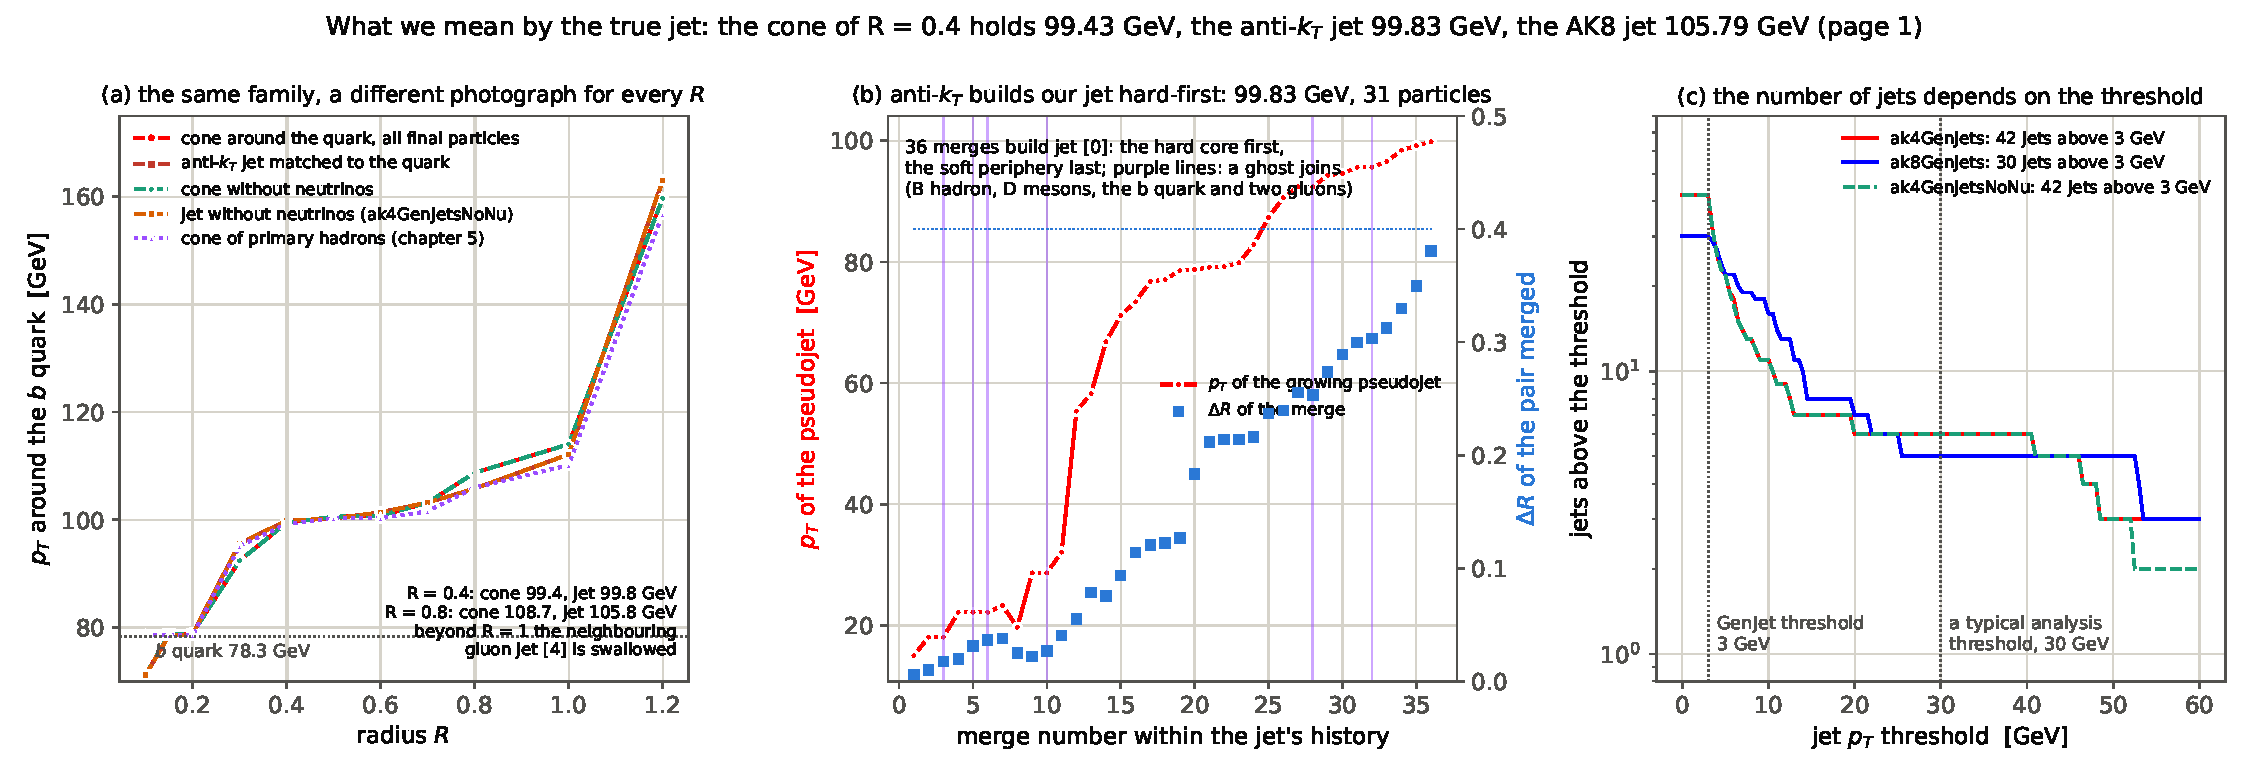
\includegraphics[page=1,width=\textwidth]{GenJet/Standalone/theory_genjets.pdf}
\caption[The profile against the radius, the ladder of our jet and the
threshold]{Page~1 of \file{theory_genjets.pdf}. (a) The \pt within $R$ of
the $b$ quark, \cref{eq:family_photograph:ptR}, for the cone of final
particles and the matched \antikt jet, with and without the neutrinos,
and for the primary hadrons of \cref{ch:children_getting_married}, from
$R=0.1$ to $1.2$. (b) The 36 merges of our \akfour jet in order, the \pt
of the pseudojet after each and the \dR of each merge, with the merges at
which a ghost joined marked. (c) The number of jets above a \pt threshold
for the three collections.}
\label{fig:family_photograph:truejet_plot}
\end{figure}

\section{Ghost-associated hadron flavour vs parton flavour}
\label{sec:family_photograph:ghost_associated_hadron_flavour_vs_parto}

The picture is taken; now the label.

\subsection{The ghosts and the \CMSSW labels}
\label{sec:family_photograph:ghosts}

Guess first: the \Bbar decayed $21\mm$ from the vertex and is nowhere
among the 749 particles. How does the experiment decide that jet [0] is a
$b$ jet and jet [3] is not? It could follow the record backwards from
every constituent, but the record of a \PYTHIA event is a tangle of
copies and the record of real data does not exist; the method has to be
one that works on the jet alone. \CMSSW's \code{JetFlavourClustering}
puts the hadron back as a \emph{ghost}: it takes the last $b$ hadron of
every decay chain, the last $c$ hadron, the partons that were handed to
the strings and the leptons from heavy-hadron decays, rescales each
four-momentum by
\begin{equation}
  p^\mu\to\varepsilon\,p^\mu,\quad\varepsilon=10^{-18},\quad
  d_{\mathrm{ghost},j}=\min\!\big((\varepsilon p_T)^{-2},p_{T,j}^{-2}\big)\frac{\dR^2}{R^2}=\frac{\dR^2}{p_{T,j}^{2}R^2},\quad
  d_{\mathrm{ghost},B}=\frac{10^{36}}{p_T^2},
  \label{eq:family_photograph:ghost}
\end{equation}
and clusters again with the ghosts among the particles. The second and
third members of \cref{eq:family_photograph:ghost} say why this works: the
distance between a ghost and any real pseudojet is the real one's, so the
ghost is filed under whatever hard pseudojet is within $R$ of it, exactly
as a soft particle would be, and its beam distance is so large that it
can never become a jet of its own; its momentum changes the jet it joins
by one part in $10^{18}$, below the precision of a double. The jet that
catches the ghost of a $b$ hadron is a $b$ jet. The labels are then two
integers per jet:
\begin{equation}
\begin{aligned}
  \hadflav&=\begin{cases}5 & \text{a $b$-hadron ghost in the jet,}\\ 4 & \text{else a $c$-hadron ghost,}\\ 0 & \text{else,}\end{cases}\\[4pt]
  \partflav&=\begin{cases}\pm5 & \text{the id of the hardest $b$-parton ghost,}\\ \pm4 & \text{else of the hardest $c$,}\\ 21,\pm1,\pm2,\pm3 & \text{else of the hardest parton,}\\ 0 & \text{none,}\end{cases}
\end{aligned}
  \label{eq:family_photograph:labels}
\end{equation}
the first unsigned and from the hadrons, the second signed and from the
partons of status 71 to 79, \PYTHIA's copies of the final partons as they
enter the hadronisation, which the standalone record carries as the rows
the strings were built from. The hadron label is what the $b$-tagging
efficiencies of \cref{ch:footprints} are measured
against~\cite{CMS:2017wtu}; the parton label is what a gluon jet and a
quark jet are told apart by in a calibration, and the two disagree
whenever a gluon splits into a heavy pair, which is a quarter of all
$b$-labelled jets in a QCD sample. Two older definitions are kept for
comparison. The \emph{physics definition} uses the hard-process partons,
status 23, as the ghosts, and the Run-1 matching took the hardest parton
within $\dR<0.3$ of the axis; both ask the hard process rather than the
hadrons, and \cref{fig:family_photograph:ghosts_sketch} shows what
happens to them in our event.

\begin{figure}[htbp]\centering
\resizebox{\textwidth}{!}{% ---------------------------------------------------------------------------
% Ghost association: (a) the Bbar0 has decayed; it is put back with its
% momentum times 1e-18, follows the clustering and lands in the jet without
% moving it; (b) the labels of CMSSW's JetFlavourClustering for the three
% b jets of our event; (c) why the physics definition (the status-23 quark)
% fails for the AK4 jet: ISR moved the hard system and the shower the family.
% Numbers: event_GenJet.lhe and standalone_genjets.log (seed 1).
% ---------------------------------------------------------------------------
\begin{tikzpicture}[x=1cm,y=1cm,
  every node/.style={font=\footnotesize},
  lab/.style={font=\scriptsize,align=center},
  head/.style={font=\small\bfseries},
  fam/.style={circle,fill=red!75!black,inner sep=0pt},
  oth/.style={circle,fill=black!40,inner sep=0pt},
  ring/.style={red!80!black,line width=1.4pt},
  ghost/.style={star,star points=5,draw=red!80!black,fill=white,thick,inner sep=1.4pt},
  flow/.style={-{Stealth[length=2mm]},thick},
  tbl/.style={font=\scriptsize,inner sep=2pt}]
% ---------------- (a) the ghost -------------------------------------------------------------------
\begin{scope}
\node[head,anchor=west] at (-0.4,4.3) {(a) the hadron comes back as a ghost};
% before: the B hadron as a particle
\node[lab,anchor=west] at (-0.4,3.7) {before the decays: the $\bar B^0$ is a particle of $78.3\,\mathrm{GeV}$};
\node[fam,minimum size=9pt] (B) at (1.2,2.9) {};
\node[lab,text=red!80!black,anchor=west] at (1.4,2.9) {$\bar B^0$ ($b\bar d$), row 1527};
\draw[flow] (1.2,2.5) -- (1.2,1.6) node[midway,right,lab] {decays: $D_s^{*-}D^{*0}\rho^+$, 15 final particles};
% after: the descendants and the ghost
\draw[ring] (1.2,0.2) circle (1.25);
\foreach \p/\s in {(1.25,0.3)/5,(1.1,0.1)/4,(1.35,0.05)/3.5,(1.0,0.45)/3,(1.5,0.4)/2.6,(0.85,-0.1)/2.4,(1.6,-0.2)/2.2,(0.7,0.55)/2,(1.3,0.75)/1.8,(0.6,-0.45)/1.6,(1.85,0.6)/1.5,(1.15,-0.6)/1.4,(1.95,-0.5)/1.3,(0.35,0.1)/1.2,(1.7,0.95)/1.1} {\node[fam,minimum size=\s pt] at \p {};}
\foreach \p/\s in {(0.5,0.95)/1.6,(2.05,0.1)/1.4,(0.3,-0.7)/1.3,(1.9,-0.95)/1.2,(0.9,1.1)/1.1,(2.2,0.8)/1.0} {\node[oth,minimum size=\s pt] at \p {};}
\node[ghost] at (1.2,0.2) {};
\draw[flow,red!80!black] (3.2,2.9) -- (3.2,1.9) node[midway,right,lab,text=red!80!black] {$p\to10^{-18}\,p$};
\node[lab,text=red!80!black,anchor=west,text width=3.3cm,align=left] at (2.6,0.3) {the ghost: same direction, no momentum; $d_{ij}=p_{T,j}^{-2}\Delta R^2/R^2$ with any real $j$, so anti-$k_T$ files it under the nearest hard pseudojet within $R$; $d_{iB}=10^{36}/p_T^2$ never wins};
\node[lab,anchor=north west,text width=5.8cm,align=left,text=black!65] at (-0.4,-1.3) {In our event the $\bar B^0$'s ghost joins the pseudojet at merge 24 of 36, $\Delta R=0.031$ from the running axis, between a photon and the $b$ quark's own ghost; the jet momentum changes by one part in $10^{18}$, below double precision.};
\end{scope}
% ---------------- (b) the labels ------------------------------------------------------------------
\begin{scope}[xshift=7.6cm]
\node[head,anchor=west] at (-0.4,4.3) {(b) the labels of the three $b$ jets (ak4)};
\foreach \x/\t in {0.1/jet,1.0/ghosts clustered,4.35/hadron,5.2/parton,6.05/physics,6.95/$\Delta R<0.3$,7.95/net} {\node[tbl,font=\scriptsize\bfseries,anchor=west] at (\x,3.6) {\t};}
\foreach \y/\j/\g/\h/\p/\f/\d/\n in {3.15/{[0] $99.8$}/{$\bar B^0$, $D^0$, $D_s^-$; $b$, $g$, $g$}/5/$+5$/0/$+5$/$+1\,b$,
                                     2.7/{[1] $94.1$}/{$\bar B^0$ (osc.), $\Xi_c^0$; $\bar b$, $g$, $g$, $g$}/5/$-5$/0/$-5$/$+1\,b$,
                                     2.25/{[2] $60.5$}/{$\bar B^0$, $\bar\Lambda_b^0$, $D^+$, $\bar D^0$; $\bar b$, $b$, $g$}/5/$-5$/0/$-5$/$0$} {
  \node[tbl,anchor=west] at (0.1,\y) {\j};
  \node[tbl,anchor=west,font=\tiny] at (1.0,\y) {\g};
  \node[tbl,fill=red!15] at (4.6,\y) {\h};
  \node[tbl] at (5.45,\y) {\p};
  \node[tbl,fill=black!8] at (6.3,\y) {\f};
  \node[tbl] at (7.3,\y) {\d};
  \node[tbl] at (8.1,\y) {\n};}
\node[lab,anchor=north west,text width=7.6cm,align=left] at (-0.4,1.55) {\textbf{hadronFlavour}: 5 if a $b$-hadron ghost is in the jet, else 4 for a $c$ hadron, else 0.\\[2pt]
 \textbf{partonFlavour}: the id of the hardest $b$-parton ghost (status 71--79), else the hardest $c$, else the hardest parton: $+5$, $-5$, or $21$, $\pm1$, $\pm2$, $\pm3$.\\[2pt]
 \textbf{physics}: the same rule with the status-23 partons as ghosts.\\[2pt]
 \textbf{net}: the sum of $\pm1$ over the $b$ hadrons, $+1$ for a $b$ quark inside ($\bar B^0$, $\Lambda_b^0$), $-1$ for a $\bar b$ ($B^0$, $B^+$, $\bar\Lambda_b^0$).};
\node[lab,anchor=north west,text width=7.6cm,align=left,text=black!65] at (-0.4,-1.3) {Jet [1] reads $+1\,b$ although it is the $\bar b$ quark's: its $B^0$ oscillated. Jet [2] holds the gluon's pair, $b$ and $\bar b$: hadronFlavour 5, net 0.};
\end{scope}
% ---------------- (c) the physics definition fails ------------------------------------------------
\begin{scope}[xshift=16.4cm]
\node[head,anchor=west] at (-0.4,4.3) {(c) where the status-23 quark points};
\draw[ring] (1.0,1.0) circle (1.2);
\node[star,star points=5,fill=red!80!black,inner sep=1.2pt] at (1.0,1.0) {};
\node[lab,text=red!80!black,anchor=north] at (1.0,0.8) {jet [0]\\ $(-1.44,-2.71)$};
\node[star,star points=5,draw=black,fill=white,inner sep=1.3pt] at (0.75,0.95) {};
\node[lab,anchor=south east] at (0.7,1.1) {$b$, status 62\\ $(-1.38,-2.73)$};
\draw[green!50!black,thick] (0.88,2.56) -- (1.12,2.80) (0.88,2.80) -- (1.12,2.56);
\node[lab,text=green!50!black,anchor=west] at (1.15,2.75) {$b$, status 23\\ $(-1.44,-2.15)$: $\Delta R=0.56$};
\draw[black!60,thin,-{Stealth[length=1.6mm]}] (1.0,2.5) -- (1.0,1.2);
\node[lab,anchor=north west,text width=4.0cm,align=left,text=black!65] at (-0.4,-0.5) {ISR gave the hard system a recoil and the shower moved the family: the hard-process quark sits outside the AK4 jet and inside the AK8 one. The CMS ``physics definition'' of Run~1 matched the status-3 parton within $\Delta R<0.3$ and would have found nothing here.};
\end{scope}
\end{tikzpicture}
}
\caption[The ghost, the labels of the three $b$ jets and the physics
definition]{The ghosts. Left: the \Bbar has decayed; it is put back with
its momentum times $10^{-18}$, \cref{eq:family_photograph:ghost}, follows
the clustering and lands in the jet without moving it. Middle: the labels
of \cref{eq:family_photograph:labels} for the three $b$-flavoured \akfour
jets of our event, with the ghosts behind each. Right: where the
status-23 $b$ quark points, $0.56$ from the jet, and why.}
\label{fig:family_photograph:ghosts_sketch}
\end{figure}

\paragraph{The numbers.} The log lists the ghosts: four $b$ hadrons, the
\Bbar of the mother at $78.26\GeV$, the oscillated \Bbar of the $\bar b$
at $81.97$, and the gluon's pair of \cref{ch:mother_gives_birth}, a
\Lbbar ($\bar u\bar d\bar b$) of $35.5$ and a \Bbar of $24.9$, both at
$\eta=-3.4$; nine $c$ hadrons, from the $D^-$ of $1.3\GeV$ to the
$\Xi_c^0$ ($dsc$) of $71.4$; $163$ partons of status 71 to 79; the two
status-23 quarks; and three leptons, $181$ ghosts in all, so that the
\akfour clustering has $930$ pseudojets to start from. Jet [0] catches
the \Bbar's ghost at its fifth merge, the $D^0$'s and the $D_s^-$'s, the
$b$ quark's and two gluons': $\hadflav=5$, $\partflav=+5$, the $\dR<0.3$
label $+5$, and the physics label $0$, because the status-23 $b$ quark
sits at $(\eta,\phi)=(-1.44,-2.15)$, $0.56$ from the jet's axis at
$(-1.44,-2.71)$. The reason is two stops back: the initial-state
radiation of \cref{ch:mother_gives_birth} recoiled the hard system and
the final-state shower moved the quark from its hard-process direction,
so that the last copy of the quark, at $(-1.38,-2.73)$, and everything
descended from it are half a unit from where the hard process put them.
The physics definition would have found this $b$ jet only with $R=0.8$,
where the status-23 ghost is inside and the label is $+5$. Jet [1], the
$\bar b$'s, has $\hadflav=5$ and $\partflav=-5$; its net flavour, the
sum of $\pm1$ over its $b$ hadrons, reads $+1$ although it is the $\bar b$
quark's jet, because the \Bz oscillated in
\cref{sec:children_producing_grandchildren:mixing} and the record holds
the \Bbar it decayed as. Jet [2], $60.45\GeV$ next to it, holds the
gluon's pair, \Lbbar and \Bbar, a $\bar b$ and a $b$: $\hadflav=5$,
$\partflav=-5$ from the harder of the two parton ghosts, net flavour
$0$. The \akeight jet of the $\bar b$ holds all three, and its physics
label is $-5$. Over four hundred decays the \Bbar's ghost lands in the
mother's \akfour jet every time, $0.062$ from the axis, with $0.20$ of its
descendants outside the jet on average and $78.2\pm0.5\%$ of the jet's
\pt from them; \hadflav is $5$ and \partflav $+5$ in $100\%$ of the
decays, and the \PYTHIA chain with \FASTJET gives $99.2$ and $99.3\%$, the
rest being decays in which the shower moved the family further than the
jet's radius. The net flavour of the mother's jet is $+1$ in $83.2\%$ and
$-1$ in $16.8\%$: the oscillation rate of
\cref{sec:children_producing_grandchildren:mixing}, read off a jet label.
Page~2 of \file{theory_genjets.pdf} (\cref{fig:family_photograph:flavour_plot})
draws the ghosts over the jets, the six labels of every jet above
$5\GeV$, and the ensemble.

\begin{figure}[htbp]\centering
\includegraphics[page=2,width=\textwidth]{GenJet/Standalone/theory_genjets.pdf}
\caption[The ghosts over the jets, the six labels of every jet, and the B
hadron against the axis]{Page~2 of \file{theory_genjets.pdf}. (a) The
ghosts of our event, $b$ hadrons, $c$ hadrons, the status-23 partons and
the status-71 partons above $3\GeV$, over the \akfour jets of the two $b$
regions. (b) One jet, six labels: \hadflav, \partflav, the physics and
the $\dR<0.3$ definitions, and the net and IFN $b$ flavours with the
heavy hadrons kept, for the 22 \akfour jets above $5\GeV$. (c) Over four
hundred decays, the \dR between the \Bbar and the axis of the mother's
jet and the share of the jet's \pt that its descendants carry.}
\label{fig:family_photograph:flavour_plot}
\end{figure}

\section{Infrared-safe flavour: flavour-$k_T$ and interleaved flavour neutralisation}
\label{sec:family_photograph:infrared_safe_flavour_flavour_k_t_and_in}

Guess first: a gluon in the periphery of the event splits into a $b\bar b$
pair so soft, half a GeV each, that nothing anyone measures changes, and
its two B~mesons land one in jet [8] and one in jet [9], two light jets of
$12$ and $11\GeV$. What are the labels now? Under
\cref{eq:family_photograph:labels} both jets have become $b$ jets, and
under the net flavour one is $+1$ and the other $-1$. An emission of
vanishing energy has changed two labels, and that is the definition of
an infrared-unsafe quantity~\cite{Sterman:1977wj,Salam:2009jx}: in a
perturbative calculation the soft $g\to b\bar b$ splitting comes with a
logarithm of the pair's mass over the jet's \pt that diverges as the pair
becomes soft, and a quantity that sees the pair inherits the divergence.
The jet's momentum does not, which is the point of \antikt; the jet's
flavour does. For the experiment, whose labels are applied to a
simulation with a finite cut-off, this is a definition and not a
disaster, and \hadflav is what the taggers are calibrated against; for a
comparison with a calculation beyond leading order, and for the $Z+b$,
$W+c$ and $t\bar t+b\bar b$ measurements that need
one~\cite{Banfi:2007gu,Gauld:2020deh}, a safe definition is needed, and
the literature has three. Flavour-$k_T$~\cite{Banfi:2006hf} changes the
distance so that a soft flavoured particle is pulled to its partner
before it can join a jet,
\begin{equation}
  \dij^{(F)}=\frac{\dR_{ij}^2}{R^2}\times\begin{cases}
    \max(k_{T,i},k_{T,j})^{\alpha}\,\min(k_{T,i},k_{T,j})^{2-\alpha} & \text{the softer of $i,j$ is flavoured,}\\
    \min(k_{T,i},k_{T,j})^2 & \text{otherwise,}\end{cases}
  \label{eq:family_photograph:fkt}
\end{equation}
with $\alpha=1$ or $2$, and the same for the beam distances with a beam
``momentum'' $k_{T,B}(y_i)=\sum_j k_{T,j}[\Theta(y_j-y_i)+\Theta(y_i-y_j)e^{y_j-y_i}]$
that sums the event on either side of the particle in rapidity: a soft
$b$ near a hard jet is as far from the jet as the jet is hard, and as
close to its soft $\bar b$ as their angle. The price is that the jets are
$k_T$ jets, irregular and different from the experiment's, which is why
it was never used on data. Flavour anti-$k_T$~\cite{Czakon:2022khx} and
flavour dressing~\cite{Gauld:2022lem} keep the \antikt jets and modify
either the distance when both are flavoured or the assignment
afterwards. Interleaved flavour neutralisation~\cite{Caletti:2022glq}
keeps the \antikt clustering exactly and adds a step before every
recombination of a flavoured pseudojet: with the neutralisation distance
\begin{equation}
  \uik=\max(p_{T,i},p_{T,k})^{\alpha}\min(p_{T,i},p_{T,k})^{2-\alpha}\,\Omega_{ik}^2,\qquad
  \Omega_{ik}^2=2\Big[\frac{\cosh(\omega\Delta y_{ik})-1}{\omega^2}-(\cos\Delta\phi_{ik}-1)\Big],
  \label{eq:family_photograph:ifn}
\end{equation}
$\alpha=2$ and $\omega=1$ for \antikt, the flavour of $i$, about to be
merged with $j$, is cancelled against every pseudojet $k$ of opposite
flavour with $\uik<u_{ij}$, closest first, each candidate's own closer
partners being settled before it; then $i$ and $j$ are merged as \antikt
would have merged them. With $\alpha=2$ the distance between the soft
$b$ and the hard core it is about to join is the core's $p_T^2$ times
their angle, and the distance between the soft $b$ and its soft $\bar b$
is their own small $p_T^2$ times their angle: the pair cancels first,
unless it is hard enough that $p_T^2\Omega^2$ of the pair exceeds that of
the merge, at which point it is a real $b\bar b$ and keeps its flavour.
$\Omega^2$ is $\dR^2$ at small angles and grows like $e^{|\Delta y|}$ at
large rapidity separation, so that a flavour far down the beam cannot
neutralise one in the barrel. The jets are the \antikt jets to the last
digit; only the labels change. The script runs
\cref{eq:family_photograph:fkt,eq:family_photograph:ifn} on the record
with the heavy hadrons kept undecayed, as the hadron-level tests of the
papers do, since a decayed B has no flavour to carry.
\Cref{fig:family_photograph:irsafety_sketch} draws the whisper and the
neutralisation.

\begin{figure}[htbp]\centering
\resizebox{\textwidth}{!}{% ---------------------------------------------------------------------------
% Infrared-safe flavour: (a) a soft g -> b bbar pair between two light jets
% relabels both under the ghost and the net definitions; (b) IFN: before the
% soft B joins its jet, its flavour is neutralised against the nearer
% opposite flavour in the distance u_ik; (c) the three distances side by
% side. Numbers: standalone_genjets.py --soft-pair 0.5 (jets [8] and [9]).
% ---------------------------------------------------------------------------
\begin{tikzpicture}[x=1cm,y=1cm,
  every node/.style={font=\footnotesize},
  lab/.style={font=\scriptsize,align=center},
  head/.style={font=\small\bfseries},
  oth/.style={circle,fill=black!40,inner sep=0pt},
  ring/.style={black!55,line width=1.2pt},
  bq/.style={star,star points=5,fill=red!80!black,inner sep=1.4pt},
  bbq/.style={star,star points=5,fill=blue!70!black,inner sep=1.4pt},
  glu/.style={decorate,decoration={coil,aspect=0.6,segment length=1.4mm,amplitude=0.7mm},green!50!black,thick},
  neut/.style={green!50!black,line width=2pt},
  box/.style={draw,rounded corners=3pt,thin,fill=gray!6,align=left,inner sep=4pt,text width=6.6cm,font=\scriptsize}]
% ---------------- (a) the whisper -------------------------------------------------------------------
\begin{scope}
\node[head,anchor=west] at (-0.4,4.3) {(a) a whisper relabels two jets};
\draw[ring] (1.0,1.2) circle (1.2); \draw[ring] (3.4,1.3) circle (1.2);
\foreach \p/\s in {(1.0,1.25)/4.5,(0.8,1.0)/3,(1.3,1.4)/2.6,(0.6,1.5)/2,(1.2,0.7)/1.8,(1.5,1.0)/1.5,(0.4,0.9)/1.3} {\node[oth,minimum size=\s pt] at \p {};}
\foreach \p/\s in {(3.4,1.35)/4.2,(3.6,1.1)/2.8,(3.15,1.6)/2.4,(3.8,1.6)/1.9,(3.2,0.8)/1.6,(3.9,1.0)/1.4,(3.5,1.9)/1.2} {\node[oth,minimum size=\s pt] at \p {};}
\node[lab,anchor=south] at (1.0,2.45) {jet [8], $12.0\,\mathrm{GeV}$};
\node[lab,anchor=south] at (3.4,2.55) {jet [9], $10.6\,\mathrm{GeV}$};
% the gluon splitting between them
\draw[glu] (2.2,-0.6) -- (2.2,0.4);
\node[lab,text=green!50!black,anchor=north] at (2.2,-0.65) {a soft gluon\\ $g\to b\bar b$};
\node[bq] (b1) at (1.75,0.85) {}; \node[bbq] (b2) at (2.65,0.95) {};
\draw[green!50!black,thin] (2.2,0.4) -- (b1); \draw[green!50!black,thin] (2.2,0.4) -- (b2);
\node[lab,text=red!80!black,anchor=north east] at (1.75,0.75) {$\bar B^0$ ($b\bar d$)\\ $0.5\,\mathrm{GeV}$};
\node[lab,text=blue!70!black,anchor=north west] at (2.65,0.85) {$B^0$ ($d\bar b$)\\ $0.5\,\mathrm{GeV}$};
\node[lab,anchor=north west,text width=5.0cm,align=left] at (-0.4,-1.5) {The pair is $0.5$ apart in $\Delta R$ and changes nothing in the event ($0.5\,\mathrm{GeV}$ in $12$). Yet: hadronFlavour $0\to5$ for both jets; net flavour $0\to+1\,b$ and $-1\,b$. The labels are not infrared safe: an emission of vanishing energy changed them.};
\end{scope}
% ---------------- (b) IFN -------------------------------------------------------------------------------
\begin{scope}[xshift=7.2cm]
\node[head,anchor=west] at (-0.4,4.3) {(b) IFN neutralises the pair first};
\draw[ring] (1.0,1.2) circle (1.2); \draw[ring] (3.4,1.3) circle (1.2);
\foreach \p/\s in {(1.0,1.25)/4.5,(0.8,1.0)/3,(1.3,1.4)/2.6,(0.6,1.5)/2,(1.2,0.7)/1.8} {\node[oth,minimum size=\s pt] at \p {};}
\foreach \p/\s in {(3.4,1.35)/4.2,(3.6,1.1)/2.8,(3.15,1.6)/2.4,(3.8,1.6)/1.9,(3.2,0.8)/1.6} {\node[oth,minimum size=\s pt] at \p {};}
\node[bq] (c1) at (1.75,0.85) {}; \node[bbq] (c2) at (2.65,0.95) {};
\draw[neut] (c1) -- (c2);
\node[lab,text=green!50!black,anchor=south] at (2.2,1.05) {$u_{ik}=0.5^2\times0.255=0.064$};
\node[oth,minimum size=3.2pt] (nb) at (1.95,0.75) {};
\node[lab,anchor=north,text=black!65] at (1.95,0.68) {$\bar n^0$, $7.4\,\mathrm{GeV}$};
\draw[-{Stealth[length=1.6mm]},red!80!black,thick,dashed] (c1) -- (nb);
\node[lab,text=red!80!black,anchor=north east] at (1.75,0.45) {$u_{ij}=7.4^2\times0.0038=0.21$:\\ the merge about to happen};
\node[lab,anchor=north west,text width=5.2cm,align=left] at (-0.4,-1.5) {Before the $\bar B^0$ ($i$, $0.5\,\mathrm{GeV}$) joins the $\bar n^0$ of $7.4\,\mathrm{GeV}$ in jet [9] ($j$, $\Delta R=0.06$), IFN looks for a pseudojet $k$ of opposite flavour with $u_{ik}<u_{ij}$, where with $\alpha=2$ $u=\max(p_{T,i},p_{T,k})^2\,\Omega^2$ and $\Omega^2=2[(\cosh\Delta y-1)-(\cos\Delta\phi-1)]$. The $B^0$: $\Delta y=0.50$, $\Delta\phi=0.02$, $\Omega^2=2[0.1276+0.0001]=0.255$, $u_{ik}=0.25\times0.255=0.064$. The merge: $\Delta y=0.04$, $\Delta\phi=0.04$, $\Omega^2=0.0038$, $u_{ij}=7.42^2\times0.0038=0.21$. $0.064<0.21$: the two flavours cancel and both jets stay flavourless. $u_{ik}$ grows as the pair's $p_T^2$ while $u_{ij}$ is set by the $7.4\,\mathrm{GeV}$ partner: above $0.9\,\mathrm{GeV}$ the pair keeps its flavour, it is then hard enough to be real.};
\end{scope}
% ---------------- (c) the three distances -------------------------------------------------------------
\begin{scope}[xshift=13.6cm]
\node[head,anchor=west] at (-0.4,4.3) {(c) the distances};
\node[box,anchor=north west] (D1) at (-0.4,3.8) {\textbf{anti-$k_T$} (the kinematics of the GenJets and of IFN)\\ $d_{ij}=\min(p_{T,i}^{-2},p_{T,j}^{-2})\,\Delta R_{ij}^2/R^2$, \quad $d_{iB}=p_{T,i}^{-2}$\\[2pt]
 \textit{our jet's first merge, $K^-$ $10.57$ GeV + $\pi^-$ $4.45$ GeV at $\Delta R=0.0056$:} $d_{ij}=10.57^{-2}\,(0.0056/0.4)^2=1.7\times10^{-6}$; $d_{iB}=10.57^{-2}=9.0\times10^{-3}$, so the pair goes first};
\node[box,below=3mm of D1.south west,anchor=north west] (D2) {\textbf{flavour-$k_T$} (Banfi, Salam, Zanderighi)\\ $d_{ij}=\Delta R_{ij}^2/R^2\times\max(k_{T,i},k_{T,j})^\alpha\min(k_{T,i},k_{T,j})^{2-\alpha}$ if the softer is flavoured,\\ $d_{ij}=\Delta R_{ij}^2/R^2\times\min(k_{T,i},k_{T,j})^2$ otherwise;\\ $d_{iB}$ the same with $k_{T,B}(y_i)=\sum_j k_{T,j}[\Theta(y_j-y_i)+\Theta(y_i-y_j)e^{y_j-y_i}]$\\[2pt]
 \textit{from the log ($\alpha=2$):} $\bar B^0$ $81.97$ GeV ($+1\,b$) + an unflavoured $1.45$ GeV at $\Delta R=0.083$, the softer unflavoured: $d_{ij}=(0.083/0.4)^2\times1.45^2=0.090$; $\bar\Lambda_b^0$ $35.75$ GeV ($-1\,b$) + $\bar B^0$ $24.93$ GeV ($+1\,b$) at $0.162$, the softer flavoured: $d_{ij}=(0.162/0.4)^2\times35.75^2=209$, a flavoured soft particle is kept apart until the end};
\node[box,below=3mm of D2.south west,anchor=north west] (D3) {\textbf{IFN} (Caola, Grabarczyk, Hutt, Salam, Scyboz, Thaler)\\ $u_{ik}=\max(p_{T,i},p_{T,k})^\alpha\min(p_{T,i},p_{T,k})^{2-\alpha}\,\Omega_{ik}^2$\\ $\Omega_{ik}^2=2\big[(\cosh\omega\Delta y-1)/\omega^2-(\cos\Delta\phi-1)\big]$, \ $\alpha=2$, $\omega=1$\\[2pt]
 \textit{the soft pair of (b):} $u_{ik}=\max(0.5,0.5)^2\times2[(\cosh0.50-1)-(\cos0.02-1)]=0.25\times0.255=0.064$; against the $\bar n^0$: $u_{ij}=7.42^2\times2[(\cosh0.04-1)-(\cos0.04-1)]=55.1\times0.0038=0.21$};
\end{scope}
\end{tikzpicture}
}
\caption[A soft $b\bar b$ pair relabels two jets; IFN neutralises it; the
three distances]{Infrared safety. Left: a soft $g\to b\bar b$ between
jets [8] and [9] of our event, one B~meson of half a GeV in each,
changes both labels under \hadflav and under the net flavour. Middle:
IFN, \cref{eq:family_photograph:ifn}, finds the opposite flavour closer
in $u$ than the merge about to happen and cancels the pair. Right: the
three distances side by side.}
\label{fig:family_photograph:irsafety_sketch}
\end{figure}

\paragraph{The numbers.} Our event has nothing to neutralise: the
\code{-v} log reports that no flavoured pseudojet found an opposite
flavour with $\uik<u_{ij}$, the gluon's pair having merged into one jet
whose net flavour is zero on its own, and the IFN labels of the 41 jets
with the heavy hadrons kept are the net labels, $+1\,b$ for jet [0],
$+1\,b$ for the oscillated jet [1], none for the rest. Flavour-$k_T$
with $\alpha=2$ makes 43 jets, the mother's with $99.83\GeV$ in 17
constituents and the $\bar b$'s with $94.49$, each with its hadron's
flavour and the two only flavoured jets of the event. The whisper is the
option \code{--soft-pair}: a $B^0$ ($d\bar b$) and a \Bbar of \pt each
and $0.5$ apart, placed between the two nearest light jets above
$5\GeV$, jets [8] and [9] at $\dR=0.64$ from each other, one hadron inside
each. At $\pt=0.5\GeV$ \hadflav becomes $5$ for both, the net flavours
$-1$ and $+1$, and IFN, before the \Bbar joins the core of jet [8] at
$u_{ij}=0.21$, finds the $B^0$ at $\uik=0.064$ and cancels the pair;
flavour-$k_T$ merges the two hadrons with each other first and leaves
both jets flavourless as well. At $\pt=1\GeV$ and above $\uik$ exceeds
$u_{ij}$, the pair is a real $b\bar b$, and all four definitions label
both jets: the scan from $0.2$ to $15\GeV$ is panel~(a) of page~3
(\cref{fig:family_photograph:irsafety_plot}). Over four hundred decays
the ensemble has $0.66$ neutralisations per event, in the periphery and
not in the two $b$ jets, whose IFN and flavour-$k_T$ labels follow the
net ones in every decay, $+1$ in $83.2\%$ for the mother's and $-1$ in
$79.2\%$ for the $\bar b$'s, the oscillations again. The candidate set
of the port, all pseudojets alive at the step with the declared jets
included, is an assumption; the reference implementation is the
\FASTJET contrib of the IFN paper, which the Python wheel of \FASTJET does
not carry, and \cref{sec:family_photograph:caveats} says so.

\begin{figure}[htbp]\centering
\includegraphics[page=3,width=\textwidth]{GenJet/Standalone/theory_genjets.pdf}
\caption[The soft-pair scan, the neutralisation distance and
flavour-$k_T$ against anti-$k_T$]{Page~3 of \file{theory_genjets.pdf}. (a)
The labels of jets [8] and [9] as a function of the \pt of each hadron of
a soft $B^0\bar B^0$ pair placed between them, under \hadflav, the net
flavour, IFN and flavour-$k_T$. (b) $\Omega^2$ of
\cref{eq:family_photograph:ifn} against $\Delta y$ for three $\Delta\phi$,
with $\dR^2$ dotted. (c) The \pt of the flavour-$k_T$ jet nearest to each
\antikt jet with the heavy hadrons kept, coloured by the IFN flavour.}
\label{fig:family_photograph:irsafety_plot}
\end{figure}

\subsection{The recipe, step by step}
\label{sec:family_photograph:step_by_step}

\Cref{fig:family_photograph:flow} is the whole stage as the script runs
it, with the numbers of our event beside each step. Read it once from top
to bottom and the \code{-v} log becomes a narrative: the input of
\cref{sec:family_photograph:choices}, the ghosts of
\cref{sec:family_photograph:ghosts}, the clustering of
\cref{sec:family_photograph:antikt} three times over, the labels, the
safe labels of
\cref{sec:family_photograph:infrared_safe_flavour_flavour_k_t_and_in}, and
the record of \cref{sec:family_photograph:record_format}. The
nearest-neighbour bookkeeping is the one branch the theory sections did
not describe: the script keeps, for every live pseudojet, its nearest
neighbour and the distance to it, recomputes only the rows that a merge
touched, and so takes a second per collection where a full matrix at
every step would take a minute; \FASTJET's $N^2$ strategy is the same
idea and its $N\ln N$ strategy a cleverer one~\cite{Cacciari:2011ma}.

\begin{figure}[htbp]\centering
\resizebox{\textwidth}{!}{% ---------------------------------------------------------------------------
% The stage as a flow chart: the steps of standalone_genjets.py on the left,
% the numbers of our event (the -v log, seed 1) on the right. Names of the
% classes and functions in grey.
% ---------------------------------------------------------------------------
\begin{tikzpicture}[x=1cm,y=1cm,
  every node/.style={font=\footnotesize},
  box/.style={draw,rounded corners=3pt,thick,fill=gray!8,align=left,inner sep=5pt,minimum height=10mm,text width=5.6cm},
  stepbox/.style={box,fill=orange!12},
  numbox/.style={draw,rounded corners=3pt,thin,fill=blue!6,align=left,inner sep=4pt,text width=8.6cm,font=\scriptsize},
  stepno/.style={draw,circle,inner sep=1pt,font=\scriptsize\bfseries,fill=orange!45,minimum size=5mm},
  flow/.style={-{Stealth[length=2.5mm,width=2mm]},thick},
  fn/.style={font=\scriptsize\ttfamily,text=black!65},
  head/.style={font=\small\bfseries}]
\node[head,anchor=west] at (-0.6,1.4) {the recipe};
\node[head,anchor=west] at (6.7,1.4) {our event (seed 1)};
\node[stepbox] (S1) at (2.5,0) {\textbf{1\; who is in the picture}\\ every final particle (status $>0$) but the \code{ignoreParticleIDs}; without the neutrinos for the NoNu collection};
\node[stepbox,below=7mm of S1] (S2) {\textbf{2\; the ghosts}\\ last $b$ and $c$ hadrons of each chain, the strings' partons (status 71--79), the status-23 partons, the leptons from heavy hadrons: momentum $\times10^{-18}$};
\node[stepbox,below=7mm of S2] (S3) {\textbf{3\; the clustering}\\ $d_{ij}=\min(p_{T}^{2p})\Delta R^2/R^2$, $d_{iB}=p_T^{2p}$, $p=-1$, $\Delta R$ in $(y,\phi)$; the smallest wins; E-scheme sums; a jet when $d_{iB}$ wins};
\node[stepbox,below=7mm of S3] (S4) {\textbf{4\; the threshold and the collections}\\ keep $p_T>3\,\mathrm{GeV}$; three times: $R=0.4$, $R=0.4$ without neutrinos, $R=0.8$};
\node[stepbox,below=7mm of S4] (S5) {\textbf{5\; the labels}\\ hadronFlavour, partonFlavour, physics, $\Delta R<0.3$, net flavour from the ghosts in each jet};
\node[stepbox,below=7mm of S5] (S6) {\textbf{6\; the safe labels}\\ heavy hadrons put back undecayed; anti-$k_T$ again with IFN replayed on its sequence; flavour-$k_T$ with its own distances};
\node[stepbox,below=7mm of S6] (S7) {\textbf{7\; write}\\ the record of chapter 6, then the jet table (one row per jet and collection) and the constituent table (one row per particle)};
\foreach \a/\b in {S1/S2,S2/S3,S3/S4,S4/S5,S5/S6,S6/S7} {\draw[flow] (\a) -- (\b);}
\foreach \n/\s in {1/S1,2/S2,3/S3,4/S4,5/S5,6/S6,7/S7} {\node[stepno] at ($(\s.west)+(-0.35,0)$) {\n};}
\node[fn,anchor=south east] at (S1.north east) {input\_rows};
\node[fn,anchor=south east] at (S2.north east) {ghost\_rows, GHOST\_RESCALING};
\node[fn,anchor=south east] at (S3.north east) {Clustering, \_row, \_run, jets};
\node[fn,anchor=south east] at (S4.north east) {JetCollection, COLLECTIONS};
\node[fn,anchor=south east] at (S5.north east) {JetCollection.flavours, composition};
\node[fn,anchor=south east] at (S6.north east) {stable\_heavy\_particles, IFN, flavour\_kt};
\node[fn,anchor=south east] at (S7.north east) {jet\_tables, read\_jet\_tables};
\node[numbox,anchor=west] (N1) at (6.7,0) {749 final particles, 5 of them neutrinos; 744 for the NoNu collection; 43 beyond $|\eta|=6$; no $\eta$ or $p_T$ cut on the input};
\node[numbox,anchor=west] (N2) at (6.7,0 |- S2) {4 $b$ hadrons ($\bar B^0$ 78.3, $\bar B^0$ 82.0 oscillated, $\bar\Lambda_b^0$ 35.5, $\bar B^0$ 24.9 GeV), 9 $c$ hadrons, 163 partons, 2 hard-process partons, 3 leptons: 181 ghosts in all};
\node[numbox,anchor=west] (N3) at (6.7,0 |- S3) {930 pseudojets, 930 steps; our jet: 36 merges from $d_{ij}=1.7\times10^{-6}$ ($K^-\pi^-$ at $\Delta R=0.006$) to $9.2\times10^{-5}$, then $d_{iB}=1.0\times10^{-4}$: $99.83\,\mathrm{GeV}$, 31 particles, 0.062 from the quark};
\node[numbox,anchor=west] (N4) at (6.7,0 |- S4) {ak4: 42 jets, 368 particles clustered, 11 above 10 GeV, 6 above 30; NoNu: 42 jets, 366 of 744; ak8: 30 jets, 600 particles; the $b$ jet $99.83$ / $99.83$ / $105.79\,\mathrm{GeV}$, the $\bar b$ jet $94.09$ / $94.09$ / $147.69$};
\node[numbox,anchor=west] (N5) at (6.7,0 |- S5) {$b$ jet: $5$ / $+5$ / $0$ / $+5$ / $+1\,b$; $\bar b$ jet: $5$ / $-5$ / $0$ / $-5$ / $+1\,b$ (oscillated); jet [2]: $5$ / $-5$ / $0$ / $-5$ / $0$ (the gluon's pair); hadronFlavour 5 for 3 jets, 4 for 2};
\node[numbox,anchor=west] (N6) at (6.7,0 |- S6) {no IFN neutralisation in the event (0.66 per decay in the ensemble, in the periphery); flavour-$k_T$: the $b$ jet $99.83\,\mathrm{GeV}$ in 17 constituents, the $\bar b$ jet $94.49$, both with their hadron's flavour};
\node[numbox,anchor=west] (N7) at (6.7,0 |- S7) {\file{event_GenJet.lhe}: 2251 rows + 330 vertex rows + 114 jet rows + 749 constituent rows; FastJet and SlowJet reproduce every jet exactly};
\end{tikzpicture}
}
\caption[The GenJet stage as a flow chart]{The steps of
\file{standalone_genjets.py} with the numbers of our event from the
\code{-v} log. The classes and functions are named in grey.}
\label{fig:family_photograph:flow}
\end{figure}

\section{Validation from official packages}
\label{sec:family_photograph:validation}

Two official sources again, and this time the first comparison is not
statistical. \FASTJET, driven from a script on the same particles, must
reproduce every jet exactly; \PYTHIA's own clustering must do the same;
and the CMS generator job of \cref{ch:ancestral_home} drew the three
collections of this chapter.

\subsection{The same particles with \FASTJET and \code{SlowJet}: the validation script}
\label{sec:family_photograph:fastjet}

\file{validate_genjets_with_fastjet.py} has two modes. In mode
\code{record} it builds the 749 particles of \file{event_Decay.lhe} and
the same $181$ ghosts as \FASTJET \code{PseudoJet}s, clusters them with
\code{JetDefinition(antikt\_algorithm, R)} and the E scheme for the three
collections, and compares jet by jet with the standalone classes: the
momenta, the constituent lists and the three labels. It then fills a
\PYTHIA event record with the same particles and runs \code{SlowJet},
\PYTHIA's own \antikt with the \code{fjcore} of \FASTJET inside, with
\code{select = 2} for the collection without neutrinos. In mode
\code{full} the hard event of \cref{ch:ancestral_home} is written to a
Les Houches file $N$ times, \PYTHIA runs the whole chain with the CP5
settings and decays on, as in
\cref{sec:children_producing_grandchildren:pythia}, and \FASTJET clusters
every event with the ghosts, taking the status-71 copy of each quark as
the axis, the choice of the \CMSSW analyser. Both modes record what
\cref{tab:family_photograph:numbers} lists, in the JSON layout of the
standalone statistics. The environment is the one of
\file{example/ME/Standalone/}, with \FASTJET added by \code{pip install
fastjet}:
\begin{minted}[linenos=false,frame=single,framesep=1.5mm,fontsize=\footnotesize]{bash}
cd example/GenJet/Standalone
PY=../../ME/Standalone/.venv/bin/python
$PY validate_genjets_with_fastjet.py                           # mode record; also --algorithm kt, ca
$PY validate_genjets_with_fastjet.py --mode full -n 2000 --standalone-stats standalone_genjet_stats.stats.json
\end{minted}
The first run takes a minute, the full chain four. The record mode
prints, for each collection,
\begin{minted}[linenos=false,frame=single,framesep=1.5mm,fontsize=\footnotesize]{text}
ak4GenJets (antikt, R = 0.4, pT > 3):
  jets: standalone 42, FastJet 42, SlowJet 42
  FastJet vs standalone, jet by jet: max |dpT| = 0.00e+00 GeV, max |dm| = 0.00e+00 GeV, identical
    constituent lists 42/42, identical (hadron, parton, physics) flavours 42/42
  SlowJet vs standalone: max |dpT| = 2.13e-14 GeV, identical constituent lists 42/42
\end{minted}
and the same for \akfournonu, for \akeight ($30$, $30$, $30$) and, with
\code{--algorithm}, for $k_T$ ($36$ jets at $R=0.8$) and Cambridge/Aachen
($35$): not a single jet, constituent or label differs, and \code{SlowJet}
agrees to the rounding of a double. This is the first stop of the journey
at which the agreement is exact rather than statistical, and it should
be: the algorithm is deterministic and
\cref{eq:family_photograph:dij,eq:family_photograph:ghost} leave nothing
to tune. The full chain, two thousand events with the shower, the
secondary scatterings and the decays all varying, is the last column but
one of \cref{tab:family_photograph:numbers}: $18.2\pm11.5$ \akfour jets
above $3\GeV$ against the $40.0$ of the fixed hadrons of the ensemble,
because the number of secondary scatterings varies and our event has
many; the mother's jet at $109.9\pm27.6\GeV$ for a quark of $95.5\pm30$,
the response $1.22\pm0.51$ with a median of $1.06$, wide because the
status-71 quark itself is soft whenever a hard gluon left it so; $7.9\GeV$
of neutrinos in the jet on average and none in $58\%$ of the events;
\hadflav $5$ in $99.2\%$. The structure is that of the ensemble, and the
numbers that the ensemble holds fixed, the shower and the underlying
event, are what the full chain spreads. The \FASTJET jets of our record
with their constituent rows are in
\file{validate_genjets_with_fastjet_record_jets.txt}.

\subsection{How CMS does it in practice: the GenJet step}
\label{sec:family_photograph:cmssw}

Nothing new has to be generated. The \code{GEN} step of
\cref{sec:ancestral_home:cmssw} runs the \code{genJetParticles} and
\code{recoGenJets} sequences after the hadron level, so that every GEN
file carries \akfour, \akfournonu and \akeight already, made by
\code{FastjetJetProducer} with \FASTJET's \antikt, the E scheme and
\code{jetPtMin = 3}; the flavour producers run later, in the
\code{PAT} step, and are not in the GEN output. \code{JitJetSW}'s
\code{genJetAnalyzer} drew the three collections as the sixth, seventh
and eighth figures of the job. From the setup of
\cref{sec:mother_gives_birth:cmssw},
\begin{minted}[linenos=false,frame=single,framesep=1.5mm,fontsize=\small]{bash}
cd CMSSW_15_0_5/src/JitJetSW/Journey/test
./runCMSDrivers_mc2024_BBbar_GEN.sh          # GEN step + genJetAnalyzer, one page per collection
\end{minted}
produces \file{genJetAnalyzer_ME_PS_MPI_Had_Decay_GenJet_out.pdf}, whose
pages 6 to 8 are \cref{fig:family_photograph:cmssw}; the copy in
\file{example/GenJet/CMSSW/} is the one used here.

\subsubsection{Reading the figures}

Page~6 is \akfour: $27$ jets, $239$ of the $634$ stable particles
clustered, the $b$ quark of status 71 at $\pt=91.74\GeV$,
$(\eta,\phi)=(-1.57,-2.08)$, matched to jet [0] of $117.79\GeV$ with $24$
constituents, $\dR=0.019$ from the quark and a response of $1.284$; the
$\bar b$ at $116.36\GeV$ and $\eta=-3.75$ matched to jet [1] of $115.94$,
$18$ constituents, response $0.996$. Page~7 is the same event without the
neutrinos: the $\bar b$'s jet is unchanged and the $b$'s has become jet
[1] of $79.82\GeV$ with $22$ constituents and a response of $0.870$, the
$37.5\GeV$ of the electron antineutrino of
\cref{sec:children_producing_grandchildren:cmssw} gone, and the two
leading jets have swapped places. Page~8 is \akeight: $28$ jets, $488$
particles clustered, the $b$'s jet at $141.10\GeV$ with $55$ constituents
and the $\bar b$'s at $121.01$ with $32$. The responses of $1.28$ and
$1.54$ for the $b$ quark are what ours are, $1.275$ and $1.351$: the
status-71 quark is the last copy before the hadronisation, soft because
the shower took its share, and the jet holds the shower's gluons back
plus the underlying event. Set the pages next to
\cref{fig:family_photograph:journey,fig:family_photograph:journey_more}.
The two are different showers of the same hard event, so the comparison
to make is \cref{tab:family_photograph:numbers}; what the pictures share
is the structure, two hard circles on the two B~hadrons, four to six
circles on the gluon and quark jets of the shower, and a scatter of
circles of a few GeV on the underlying event, $27$ in one event and $42$
in the other, with hollow particles everywhere between them that no
circle above $3\GeV$ reached.

\begin{figure}[htbp]\centering
\includegraphics[page=6,width=\textwidth]{GenJet/CMSSW/genJetAnalyzer_ME_PS_MPI_Had_Decay_GenJet_out.pdf}\\[2mm]
\includegraphics[page=7,width=0.495\textwidth]{GenJet/CMSSW/genJetAnalyzer_ME_PS_MPI_Had_Decay_GenJet_out.pdf}\hfill
\includegraphics[page=8,width=0.495\textwidth]{GenJet/CMSSW/genJetAnalyzer_ME_PS_MPI_Had_Decay_GenJet_out.pdf}
\caption[The generator-level jets of the event in \CMSSW]{Stage~6 of our
event in \CMSSW, drawn by the \code{genJetAnalyzer} of \code{JitJetSW}:
\akfour (top), \akfournonu (bottom left) and \akeight (bottom right).
Every jet above $3\GeV$ is a circle of radius $R$, the $b$ jet red and
the $\bar b$ jet blue with their constituents, the leading other jets in
colour, the stable particles in no jet hollow, and the status-71 $b$
quarks as stars; the header gives the quark-to-jet matching with \dR and
the response. The same stage of the standalone record is
\cref{fig:family_photograph:journey,fig:family_photograph:journey_more}.}
\label{fig:family_photograph:cmssw}
\end{figure}

\section{Our jet at this stage: the reference GenJet we will compare to forever}
\label{sec:family_photograph:our_jet_at_this_stage_the_reference_genj}

The photograph is taken: jet [0] of \akfour, $99.83\GeV$, $31$ particles,
$\hadflav=5$. Every reconstructed jet from \cref{ch:the_inn} on will be
matched to it within $\dR<0.2$ and its response measured against it, and
the ledger of this stop records what it holds.

\begin{table}[htbp]\centering\small
\caption[Kinematics of the two $b$ quarks, their jets and their cones]{Kinematics
of the two $b$ quarks and of the jets of the three collections matched to
them, from \file{event_GenJet.lhe} as printed by
\file{standalone_genjets.py}, with the cone of the same radius around the
quark for comparison. ``Response'' is $\pt(\mathrm{jet})/\pt(b)$ with
the last copy of the quark; \dR is the distance in $(\eta,\phi)$ from
the quark to the jet axis; the labels are \hadflav, \partflav, the
physics and the $\dR<0.3$ definitions, and the net $b$ flavour.}
\label{tab:family_photograph:kinematics}
\scriptsize\setlength{\tabcolsep}{3pt}
\begin{tabular}{llrrrrrl}\toprule
 & & $\pt$ [GeV] & $m$ [GeV] & $n$ & \dR & resp. & labels \\ \midrule
$b$ & the quark (row 719, last copy) & $78.29$ & $4.80$ & $1$ & & & \\
    & its \Bbar (row 1527, chapter 6) & $78.26$ & $5.28$ & $1$ & $0.06$ & & \\
    & the cone $\dR<0.4$, final (chapter 6) & $99.43$ & $14.59$ & $31$ & & $1.270$ & \\
    & \akfour jet [0] & $99.83$ & $14.83$ & $31$ ($17$ ch.) & $0.062$ & $1.275$ & $5$, $+5$, $0$, $+5$, $+1$ \\
    & \quad ch.\ hadrons / photons / neutral had. & $68.1$ / $22.8$ / $9.0$ & & $17$ / $13$ / $1$ & & & \\
    & \quad the \Bbar's descendants / neutrinos & $78.26$ / $0$ & & $15$ / $0$ & & & \\
    & \akfournonu jet [0] & $99.83$ & $14.83$ & $31$ & $0.062$ & $1.275$ & the same \\
    & the cone $\dR<0.8$ (chapter 6) & $108.73$ & $42.14$ & $51$ & & $1.389$ & \\
    & \akeight jet [1] & $105.79$ & $27.43$ & $47$ ($25$ ch.) & $0.078$ & $1.351$ & $5$, $+5$, $+5$, $+5$, $+1$ \\ \midrule
$\bar b$ & the quark (row 708, last copy) & $72.50$ & $4.80$ & $1$ & & & \\
    & its \Bbar (row 1590, oscillated) & $81.97$ & $5.28$ & $1$ & $0.02$ & & \\
    & the cone $\dR<0.4$ & $93.02$ & & $18$ & & $1.283$ & \\
    & \akfour jet [1] & $94.09$ & $17.83$ & $18$ ($8$ ch.) & $0.035$ & $1.298$ & $5$, $-5$, $0$, $-5$, $+1$ \\
    & \akfour jet [2], the gluon's pair & $60.45$ & $11.79$ & $29$ ($14$ ch.) & $0.87$ & & $5$, $-5$, $0$, $-5$, $0$ \\
    & \akeight jet [0], both of the above & $147.69$ & $75.40$ & $57$ ($28$ ch.) & $0.361$ & $2.037$ & $5$, $-5$, $-5$, $21$, $+1$ \\ \midrule
\multicolumn{2}{l}{$b$ jet + $\bar b$ jet (\akfour): $|\vec p_T|$, $\Sigma|\pt|$, $\Delta\phi$, $m$} & $16.9$, $193.9$ & $302$ & & & $2.98$ & \\
\bottomrule
\end{tabular}
\end{table}

\Cref{tab:family_photograph:kinematics} and
\cref{fig:family_photograph:journey} say what the record means for the
ledger, and the lesson has two halves. The photograph and the cone agree
to half a percent, $99.83$ against $99.43\GeV$, because \antikt with
$R=0.4$ around a family this collimated is a cone around the family's own
axis; the difference, four soft particles at the border, is the
$0.06$ by which the axis moved from the quark to the hadron's
descendants, and over four hundred decays the jet exceeds the cone by
$0.84\pm0.59\GeV$. The jet is $68.1\GeV$ of charged hadrons, $22.8$ of
photons and $9.0$ of neutral hadrons, the proportions the detector of
\cref{ch:crossing_the_border} will take apart, and nothing else: no
lepton and no neutrino, so that the jet without neutrinos is the same
jet and the response of $1.275$ is what every later stage will be
measured against. The second half is what the photograph does not show.
The response of $1.275$ is not the family's, which carries $78.3$ of the
quark's $78.3\GeV$, but the picture's, which added $21.5\GeV$ of gluons
and underlying event within $R=0.4$ around it, and the $\bar b$ quark's
\akeight jet, with a response of $2.04$, shows how far that can go when a
second family sits within $R$: the gluon's $b\bar b$ pair of
\cref{ch:mother_gives_birth}, a jet of $60\GeV$ in its own right at
$\dR=0.87$ from the $\bar b$ quark, is inside the large circle and
outside the small one. The ensemble says the rest: with neutrinos the
photograph is stable to half a GeV, $99.63\pm0.49$; without them, which
is the one CMS uses, it is $91.93\pm12.12$, and that $12\GeV$, a
sixth of the decays with more than $5\GeV$ of neutrino, is the first
irreducible term of the resolution of a $b$ jet, taken at this stop and
carried to the end.

\begin{figure}[htbp]\centering
\includegraphics[page=4,width=\textwidth]{GenJet/Standalone/theory_genjets.pdf}
\caption[The family through the stages and its photographs, the
composition of the jet, and the response]{Page~4 of
\file{theory_genjets.pdf}. (a) The \pt of the family through the stages,
partons, primary hadrons, final particles, and the three photographs,
\akfour, \akfournonu and \akeight, for our event and for the mean of 400
decays, with the \CMSSW event's numbers. (b) What the \akfour jet is made
of: charged hadrons, photons, neutral hadrons, leptons and neutrinos, for
our event, the ensemble and the \PYTHIA chain. (c) The response
$\pt(\mathrm{jet})/\pt(b)$ over 400 decays for the three collections and
over the \PYTHIA chain, with our event and the \CMSSW event marked.}
\label{fig:family_photograph:our_jet_plot}
\end{figure}

\begin{figure}[htbp]\centering
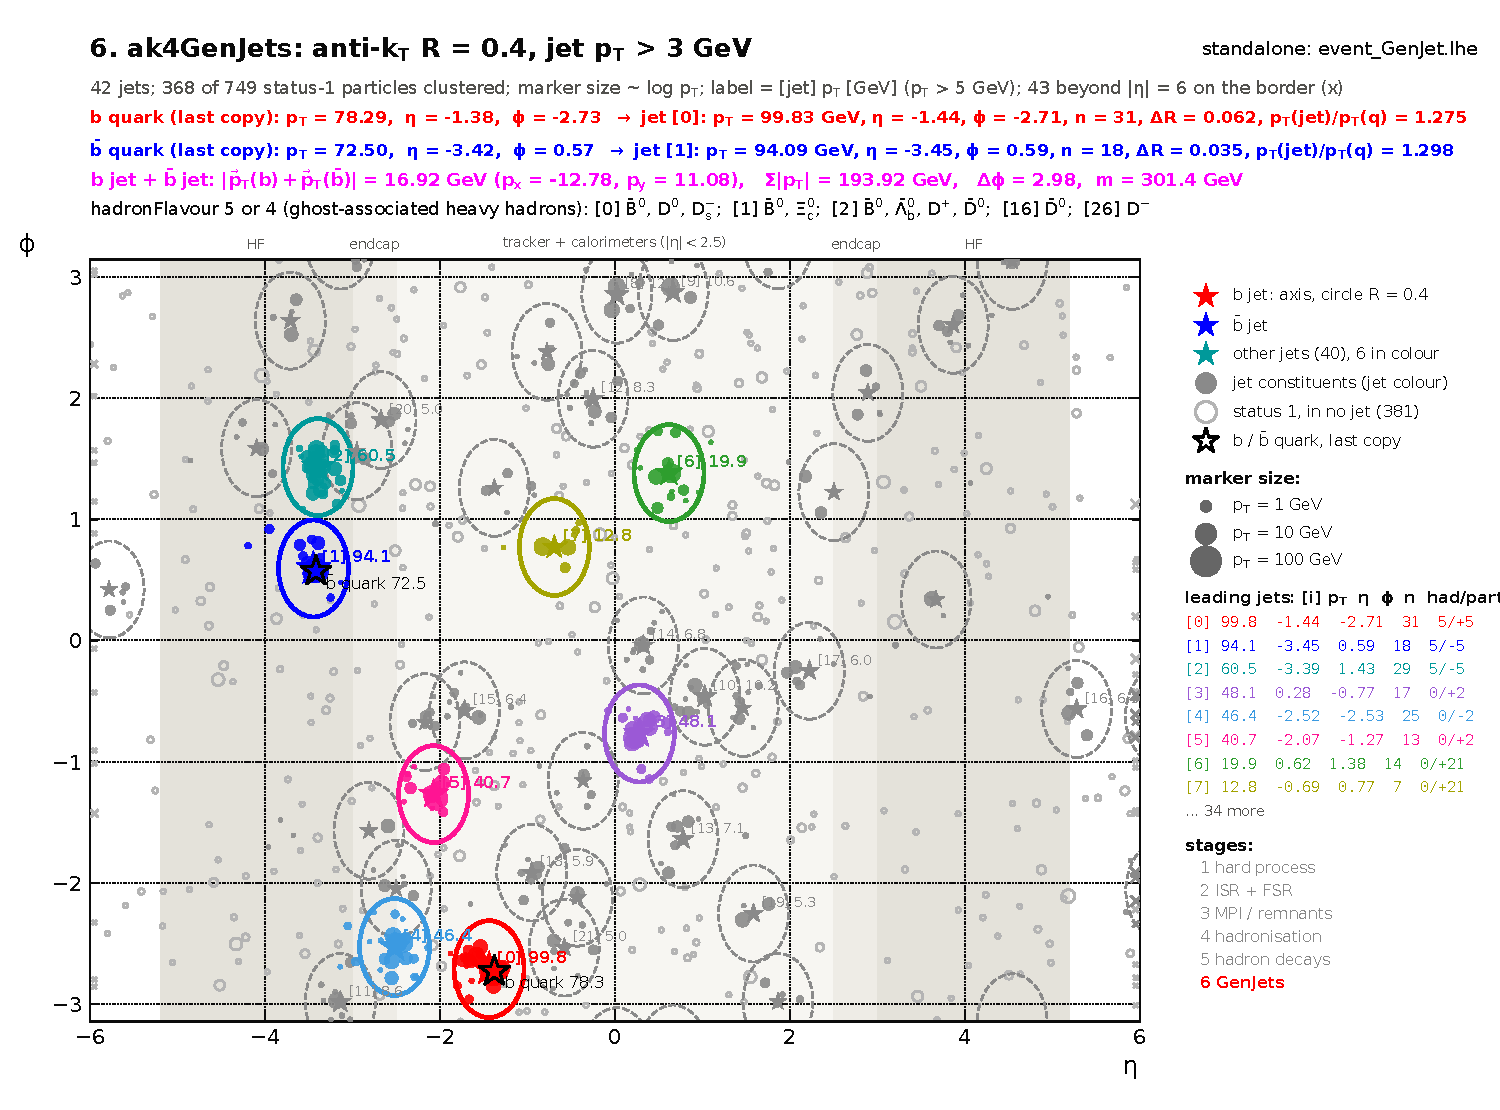
\includegraphics[width=\textwidth]{GenJet/journey_GenJet.pdf}
\caption[The \akfour jets of the event in the $(\eta,\phi)$ plane]{The
\akfour collection of our event, drawn by
\file{example/GenJet/plot_journey_GenJet.py} from
\file{example/GenJet/event_GenJet.lhe} in the layout of
\cref{fig:family_photograph:cmssw}. The 42 jets above $3\GeV$ are circles
of radius $0.4$, the $b$ jet red at $(-1.44,-2.71)$ and the $\bar b$ jet
blue at $(-3.45,0.59)$, the next six in colour, the rest grey with their
constituents; the 381 particles in no jet are hollow and the last copies
of the quarks black stars. The header gives the quark-to-jet lines with
\dR and the response, the two-jet system, and the heavy hadrons behind
each \hadflav label; the margin lists the leading jets with their two
labels.}
\label{fig:family_photograph:journey}
\end{figure}

\begin{figure}[htbp]\centering
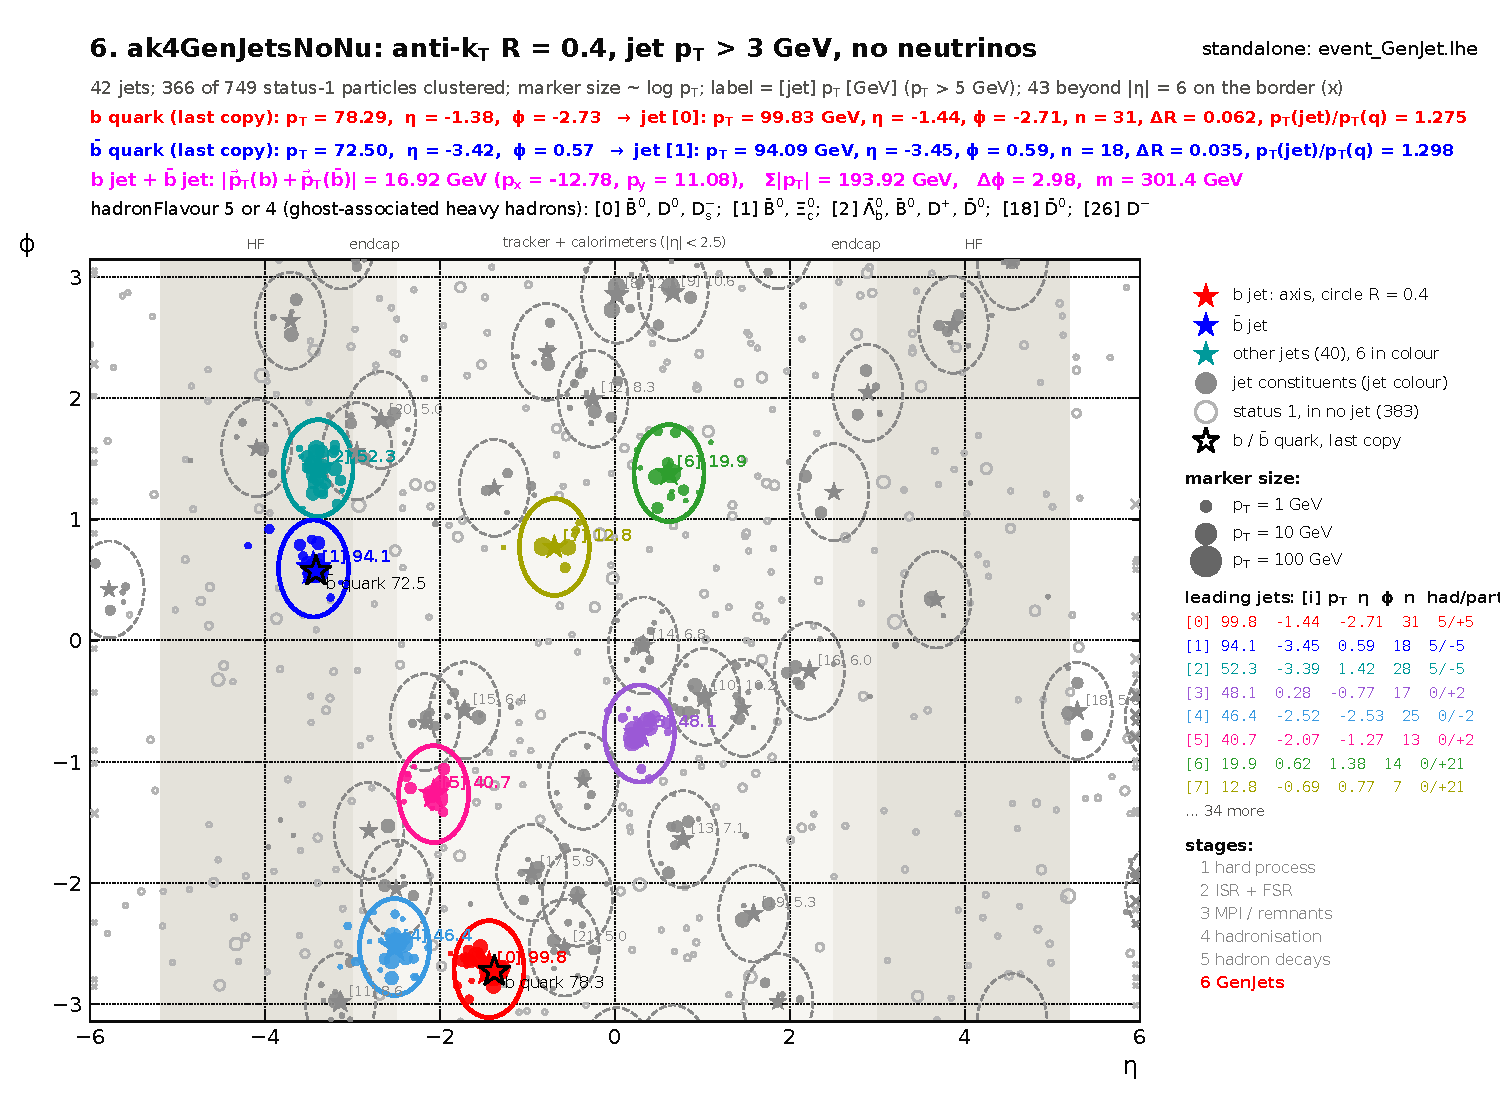
\includegraphics[width=0.84\textwidth]{GenJet/journey_GenJet_nonu.pdf}\\[1mm]
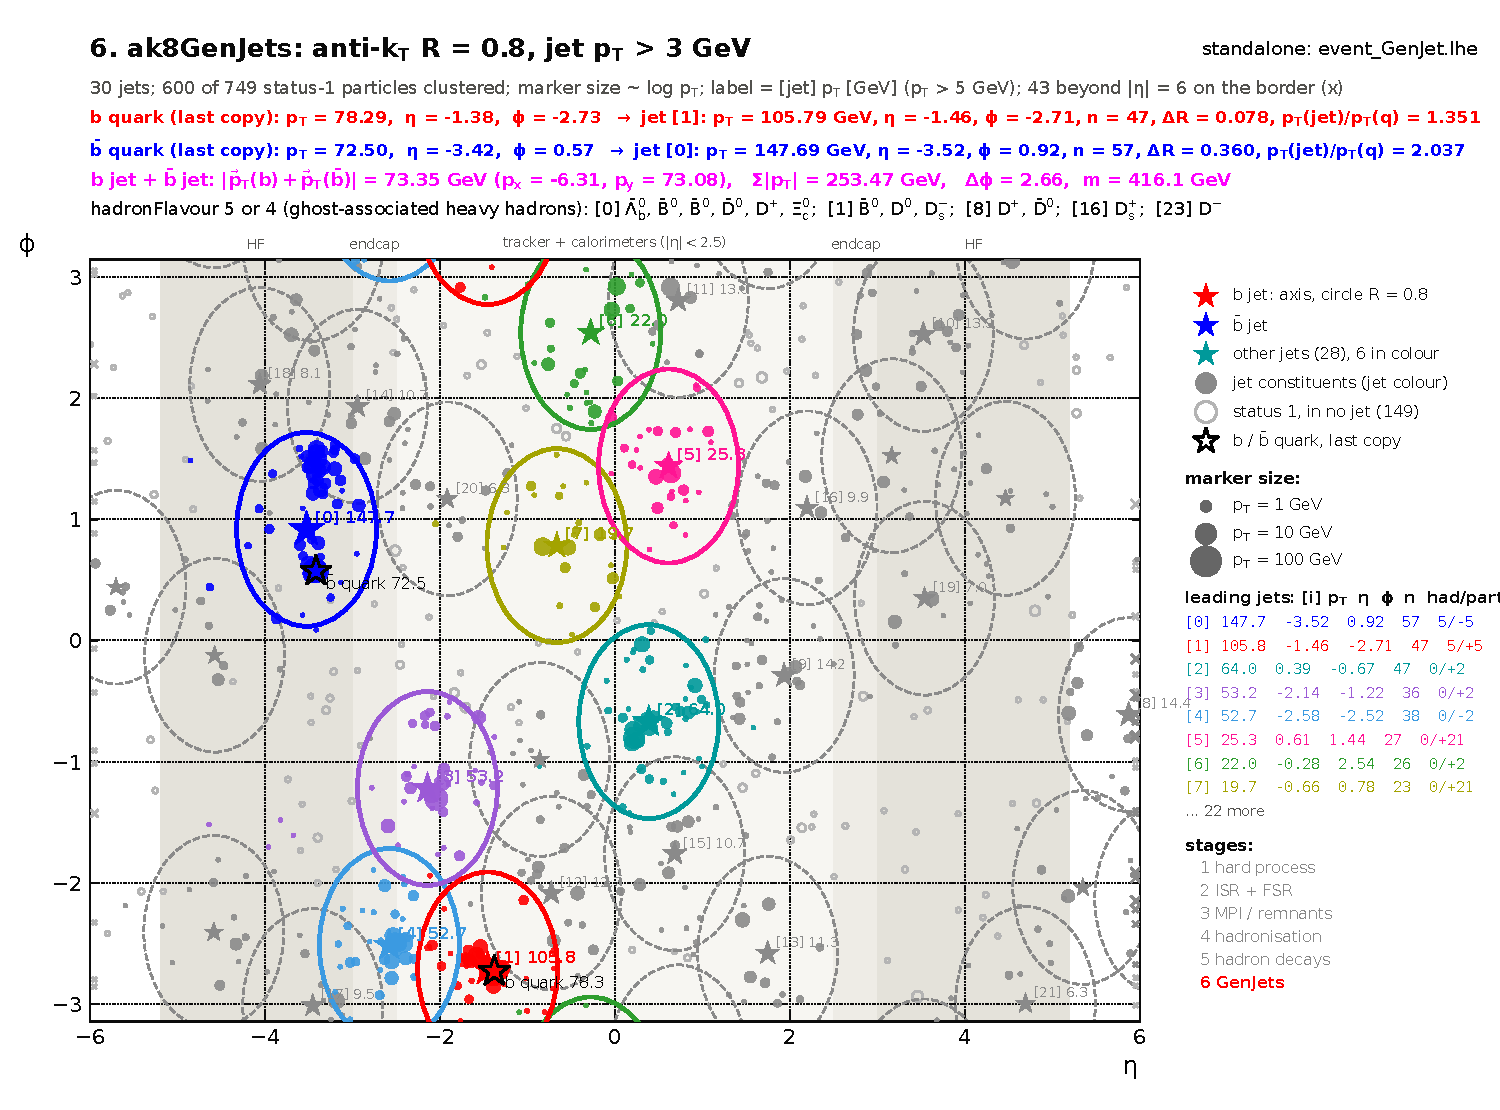
\includegraphics[width=0.84\textwidth]{GenJet/journey_GenJet_ak8.pdf}
\caption[The \akfournonu and \akeight jets of the event]{The other two
collections of our event, \akfournonu (top) and \akeight (bottom), in the
same layout. Without the neutrinos the two $b$ jets are unchanged and the
gluon pair's jet [2] loses its $8.1\GeV$ neutrino; with $R=0.8$ the
$\bar b$'s jet swallows the pair, $147.69\GeV$ and three B~hadrons at
$\dR=0.36$ from the quark, and the $b$'s grows to $105.79$.}
\label{fig:family_photograph:journey_more}
\end{figure}

The ledger gets the photograph. The first row is the last one of
\cref{ch:children_producing_grandchildren}; the three jets are new, and
the \akfournonu row is the one every later stage is corrected towards.

\begin{ledger}{The Family Photograph}
  \ledgerrow{$b$ family after the decays ($\dR<0.4$, final)}{99.43}{14.59}{31}{--}
  \ledgerrow{\akfour jet [0], the photograph}{99.83}{14.83}{31}{$+0.40$}
  \ledgerrow{\quad \akfournonu jet [0], the reference}{99.83}{14.83}{31}{$0.00$}
  \ledgerrow{\quad of which charged hadrons}{68.09}{--}{17}{--}
  \ledgerrow{\quad of which the \Bbar's descendants}{78.26}{5.28}{15}{--}
  \ledgerrow{\quad mean of 400 decays, with neutrinos}{99.63}{14.11}{25.7}{--}
  \ledgerrow{\quad mean of 400 decays, without}{91.93}{13.29}{25.2}{$-7.70$}
  \ledgerrow{\akeight jet [1], the same family at $R=0.8$}{105.79}{27.43}{47}{$+5.96$}
\end{ledger}

\section{What this stage is, and what it is not}
\label{sec:family_photograph:caveats}

The agreement in \cref{tab:family_photograph:numbers} with \FASTJET is
exact, and the parts of the chapter that are not a port of \FASTJET
carry their caveats:
\begin{itemize}
  \item \textbf{A photograph, not a truth.} The generator-level jet is
    a definition, and a different generator, tune or decay model gives a
    different one for the same hard event; the $21.5\GeV$ of gluons and
    underlying event in our jet are \PYTHIA's shower and CP5's
    multiparton interactions, and \cref{ch:paying_for_uninvited} will
    correct the reconstructed jet towards \emph{this} picture, not
    towards the quark.
  \item \textbf{The \akfournonu convention is CMS's.} ATLAS calibrates
    to jets that include the neutrinos from hadron decays and treats the
    difference in its $b$-jet uncertainties; a response quoted without
    saying which photograph it refers to is $8\%$ ambiguous for a $b$
    jet.
  \item \textbf{The ghost partons of \CMSSW are a selection.}
    \code{Pythia8PartonSelector} takes status 71 to 79, which the
    standalone record has as the rows the strings were built from; the
    ``physics'' partons of \CMSSW's \code{physicsPartons} collection are
    approximated here by the status-23 partons alone, and the
    \code{hadronFlavourHasPriority} switch that lets a $b$ hadron
    override a light \partflav is left off, as in the default
    configuration.
  \item \textbf{The sign of \partflav for a jet with both.} Jet [2] holds
    a $\bar b$ and a $b$ parton ghost and reads $-5$ from the harder; a
    jet from $g\to b\bar b$ carries one sign by that accident, as it does
    in \CMSSW.
  \item \textbf{IFN is a port of a paper, not of the code.} The
    candidate set, the recursion and the treatment of jets already
    declared follow the description of \cite{Caletti:2022glq}; the
    reference is the \FASTJET contrib, which could not be run here. The
    neutralisation of the soft pair and the absence of one in our event
    do not depend on those details; a corner case might.
  \item \textbf{Flavour-$k_T$ without beam flavour.} The beams carry no
    flavour in the port; the paper's treatment of an initial-state
    heavy quark is not needed for a $b\bar b$ final state from light
    partons.
  \item \textbf{Hadron level with the heavy hadrons kept.} The safe
    definitions are run with the last $b$ and $c$ hadrons put back in
    place of their descendants, as the papers' hadron-level tests do;
    the neutrinos of their decays are then inside the hadron, and the
    jets of that run differ from \akfour at the border by a few hundred
    MeV.
  \item \textbf{The response is to the last copy.} $1.275$ divides by
    the quark of status 62 after the shower; the hard-process quark had
    $113.2\GeV$ and the response to it would be $0.88$. \CMSSW divides by
    the status-71 copy, the same object; the full chain's spread of $0.5$
    in that ratio is the denominator's, not the jet's.
  \item \textbf{One event is one sample.} The $42$ jets and the
    $0.40\GeV$ between jet and cone are this event's; the ensemble has
    $40.0\pm2.2$ and $0.84\pm0.59$, and the \CMSSW event $27$ jets.
\end{itemize}

\section{Further reading}
\label{sec:family_photograph:further_reading}
The \antikt algorithm is \cite{Cacciari:2008gp} and its implementation,
with the $N^2$ and $N\ln N$ strategies, the \FASTJET
manual~\cite{Cacciari:2011ma}; its ancestors are the $k_T$ algorithms of
\cite{Catani:1993hr,Ellis:1993tq} and the Cambridge/Aachen algorithm of
\cite{Dokshitzer:1997in,Wobisch:1998wt}, and the jet area that the same
ghosts measure is \cite{Cacciari:2008gn}. Infrared and collinear safety
begins with \cite{Sterman:1977wj} and is explained for jets in Salam's
``Towards jetography''~\cite{Salam:2009jx}. The infrared-safe flavour
definitions are flavour-$k_T$~\cite{Banfi:2006hf} with its application to
heavy-quark jets~\cite{Banfi:2007gu}, flavour anti-$k_T$~\cite{Czakon:2022khx},
flavour dressing~\cite{Gauld:2022lem} and interleaved flavour
neutralisation~\cite{Caletti:2022glq}, with the NNLO view of
\cite{Caletti:2022hnc} and the QCD-aware truth labelling of
\cite{Buckley:2015gua}; what they are needed for is the $Z+b$
calculation of \cite{Gauld:2020deh}. The experiment's side is the
$b$-tagging paper of CMS~\cite{CMS:2017wtu}, whose efficiencies are
measured against \hadflav, and the jet energy scale
paper~\cite{CMS:2016lmd}, whose reference is the jet without neutrinos;
the generators' side is \PYTHIA~8.3's guide~\cite{Bierlich:2022pfr} for
the status codes and \code{SlowJet}.

\begin{pitfalls}
\begin{itemize}[nosep]
  \item \textbf{Rapidity, not pseudorapidity.} \antikt measures \dR in
    $y$; the pictures are drawn in $\eta$. For a pion the two agree; a
    B~meson of $0.5\GeV$ placed at $y=0.1$ sits at $\eta=0.85$. The soft
    pair of the infrared test is placed in $y$, and a first version of
    the film drew it in $\eta$, outside both jets.
  \item \textbf{The cone is not the jet.} Same radius, same family,
    $99.43$ against $99.83\GeV$; the axis moved by $0.06$ and four soft
    particles changed sides. Compare a jet with a jet.
  \item \textbf{Three collections, three answers.} $99.83$, $99.83$ and
    $105.79\GeV$ in our event, and in the \CMSSW event $117.8$, $79.8$ and
    $141.1$. A response without the name of its collection is not a
    number.
  \item \textbf{The $3\GeV$ threshold is in the GEN file.} \akfour has
    $42$ jets here, and \code{slimmedGenJets} in a MiniAOD file keeps
    those above $8\GeV$; a matching to the nearest GenJet depends on
    which file one reads.
  \item \textbf{\hadflav has no sign and \partflav has one.} $5$ against
    $+5$ and $-5$; a $b$ jet from $g\to b\bar b$ reads $5$ from the
    hadrons and one sign from the harder parton.
  \item \textbf{The status-23 quark is not where the jet is.} $0.56$
    away in our event; the physics definition and the Run-1 $\dR<0.3$
    matching to status-3 partons find nothing. Use the ghosts.
  \item \textbf{A ghost must not merge into a jet of its own.} The beam
    distance of a ghost is $10^{36}/p_T^2$; with $k_T$ ($p=+1$) the
    ghosts cluster among themselves first and still end in the nearest
    hard jet, which is correct, but the step count doubles.
  \item \textbf{Net flavour reads the oscillation.} $+1$ for the
    $\bar b$ quark's jet; $17\%$ of the mother's decays read $-1$. The
    net flavour of a jet is the hadron's at decay, not the quark's.
  \item \textbf{The gluon's pair is one jet at $R=0.4$ and part of the
    $\bar b$'s at $0.8$.} Jet [2] with \hadflav $5$ and net $0$ is a
    $g\to b\bar b$ jet, the kind a tagger calibrated on single-$b$ jets
    misjudges; at $R=0.8$ it disappears into the $\bar b$'s jet, which
    then reads three B~hadrons.
  \item \textbf{Infrared safety is about labels too.} The jet's \pt is
    safe under a soft pair, its \hadflav is not; the scan of
    \cref{fig:family_photograph:irsafety_plot} is a one-line test to run
    on any new definition.
  \item \textbf{IFN with $\alpha=2$ ignores the soft one's \pt.}
    $\max(p_T)^2\Omega^2$ for both the merge and the candidate; what
    decides is which hard object the soft flavour is closer to in
    $\Omega^2$, scaled by that object's $p_T^2$.
  \item \textbf{Response to which quark?} $1.275$ to the last copy,
    $0.88$ to the hard-process quark; the full chain's response has a
    width of $0.5$ because its denominator moves.
  \item \textbf{Which Python?} The standalone, plotting and animation
    scripts run with a \code{python3} that has NumPy and matplotlib; the
    validation script needs the virtual environment of
    \file{example/ME/Standalone/} with \FASTJET installed by \code{pip}.
\end{itemize}
\end{pitfalls}

\begin{exercises}
\item \textbf{Run it.} Run \file{standalone_genjets.py} and confirm $42$
  \akfour jets, $99.83\GeV$ and $31$ constituents for jet [0],
  $\hadflav=5$ and $\partflav=+5$. Run \code{--algorithm kt} and
  \code{ca} and count the jets above $3$, $10$ and $30\GeV$; which
  algorithm makes the most jets above $3\GeV$ and why?
\item \textbf{The distance.} From the log's first merge, $K^-$ of
  $10.567\GeV$ and $\pi^-$ of $4.451$ at $\dR=0.006$, reproduce
  $\dij=1.74\times10^{-6}$ with \cref{eq:family_photograph:dij}; then
  compute \diB for the finished jet and check that it exceeds the last
  merge's \dij. What would the first merge have been with $p=+1$?
\item \textbf{The profile.} With \code{--radius} from $0.1$ to $1.2$
  reproduce panel~(a) of \cref{fig:family_photograph:truejet_plot} for
  the jet, and from the record the cone; at which $R$ does the gluon jet
  [4] enter, and what is its \pt?
\item \textbf{The threshold.} Count the \akfour jets above $5$, $8$,
  $15$ and $20\GeV$ from the jet table; how many of the $42$ have a
  single constituent, and what are they?
\item \textbf{The neutrino.} Run the decay script of
  \cref{ch:children_producing_grandchildren} with \code{--seed 4}, then
  this script on its output, and reproduce $99.6$ and $90.2\GeV$ for the
  two \akfour collections. From \file{standalone_genjet_stats.stats.json}
  reproduce $91.93\pm12.12$, the $54\%$ without a neutrino and the $37\%$
  above $5\GeV$.
\item \textbf{The ghost.} Compute $d_{\mathrm{ghost},j}$ and
  $d_{\mathrm{ghost},B}$ of \cref{eq:family_photograph:ghost} for the
  \Bbar's ghost against the pseudojet of $22.16\GeV$ it joined at
  $\dR=0.031$; then change \code{GHOST\_RESCALING} to $10^{-6}$ and find
  the first jet whose \pt changes in the sixth digit.
\item \textbf{The labels.} From the jet table reproduce the labels of
  jets [0], [1] and [2] from the ghosts listed with each; then explain
  from the record why jet [1] reads net $+1\,b$ and jet [2] reads $0$.
\item \textbf{The physics definition.} From rows 6 and 719 of the record
  compute the \dR between the status-23 $b$ quark and its last copy, and
  from \file{event_PS.lhe} find the branching that moved it most. For
  which $R$ does the status-23 ghost enter the $b$ jet?
\item \textbf{The whisper.} Run \code{--soft-pair} at $0.2$, $0.5$, $1$,
  $2$ and $5\GeV$ and tabulate the four labels of jets [8] and [9];
  reproduce $\uik=0.064$ and $u_{ij}=0.21$ at $0.5\GeV$ from
  \cref{eq:family_photograph:ifn} and the log's positions. At what \pt
  does IFN stop neutralising, and why there?
\item \textbf{$\Omega^2$.} Plot $\Omega^2$ of \cref{eq:family_photograph:ifn}
  against $\dR^2$ for $\Delta\phi=0$ and $\Delta y$ from $0$ to $3$, and
  find the $\Delta y$ at which the two differ by a factor two; what does
  that do to a $\bar b$ hadron at $\eta=-3.4$ as a candidate for the
  mother's $b$ at $-1.4$?
\item \textbf{Flavour-$k_T$.} From \cref{eq:family_photograph:fkt} explain
  why the two soft hadrons of the whisper merge with each other before
  either joins a jet, and why with $\alpha=1$ the same holds; then
  compare the flavour-$k_T$ jet of the mother, $17$ constituents, with
  the \antikt one, $31$: which particles differ?
\item \textbf{The ensemble.} From the statistics file compute the mean
  and the width of the jet minus the cone at $R=0.4$ and at $0.8$,
  reproduce $0.84\pm0.59$ and $-2.60\pm0.62$, and explain the sign at
  $0.8$.
\item \textbf{\FASTJET by hand.} Run the validation script, then change
  the recombination scheme in it to \code{pt\_scheme} and find how far
  the jet masses move; then run \code{SlowJet} with \code{massSet = 0}
  and explain the change in the rapidities.
\item \textbf{The \CMSSW pages.} From the headers of pages 6 to 8
  reproduce the responses $1.284$, $0.870$ and $1.538$ and the $37.5\GeV$
  of neutrino from the difference of the first two; then explain why the
  $\bar b$'s jet has the same \pt with and without the neutrinos.
\item \textbf{Film it.} Run the animation with \code{--scene whisper}
  and, from the \code{-v} log of \code{--soft-pair 0.5}, predict before
  watching the two distances that the neutralisation line will quote.
\end{exercises}

\subsection*{Open problems in the context of Phase-2 LHC}
\label{sec:family_photograph:open_problems}

The photograph is a convention, and the High-Luminosity LHC will stretch
every convention in it: jets at two hundred collisions per crossing need
a reference whose own ambiguities are smaller than the corrections of
\crefrange{ch:paying_for_uninvited}{ch:the_receipt}, and measurements of
$t\bar t+b\bar b$, $Z+b$ and $H\to b\bar b$ at the precision of
\cite{Azzi:2019yne} need a flavour definition that a calculation can
share with the experiment. Each of the following can be started with
the scripts of this chapter.
\begin{enumerate}
  \item \textbf{A safe flavour label in the experiments.} \hadflav is
    what CMS and ATLAS calibrate their taggers against, and it is not
    infrared safe; IFN~\cite{Caletti:2022glq}, flavour
    anti-$k_T$~\cite{Czakon:2022khx} and flavour dressing~\cite{Gauld:2022lem}
    are, and keep the \antikt jets, so that for the first time the
    experiments could label their simulated jets with the definition a
    NNLO calculation~\cite{Gauld:2020deh,Caletti:2022hnc} uses. The open
    question is practical: how often do the labels differ in a $b$-jet
    sample, and in which jets? With the ensemble's \code{net} and
    \code{ifn} entries and the \code{--soft-pair} scan, measure the
    fraction of jets whose \hadflav and IFN labels disagree as a function
    of the jet \pt and of the $g\to b\bar b$ rate, which
    \cref{ch:mother_gives_birth} can vary; the Phase-2 question is
    whether a tagger calibrated against a safe label loses efficiency on
    the gluon-splitting jets it no longer counts as $b$.
  \item \textbf{The neutrino in the reference.} CMS corrects to the jet
    without neutrinos and ATLAS to the jet with them, and the
    difference, $8\GeV$ on average and $12$ in width for the mother's
    jet, is absorbed in $b$-jet energy scale uncertainties and in the
    regressions of \cite{CMS:2019uxx}. At the HL-LHC the top-quark mass
    and the $H\to b\bar b$ signal strength will be limited by exactly
    this term~\cite{Azzi:2019yne}. From the ensemble, measure how much of
    the $12\GeV$ a photograph that keeps the neutrino's direction but
    not its energy, or one that adds the soft lepton's momentum back,
    would recover; the question is which reference definition minimises
    the data-to-simulation uncertainty of a $b$ jet rather than its
    resolution.
  \item \textbf{The radius at two hundred pileup.} The profile of
    \cref{eq:family_photograph:ptR} rises by $9\GeV$ from $R=0.4$ to
    $0.8$ for our family and the underlying event adds a GeV per tenth
    of a unit; at the HL-LHC the pileup of \cref{ch:crowd_on_the_road}
    adds $0.6\GeV$ per unit of area per collision before subtraction.
    With the profile of the ensemble and the pileup density of
    \cref{ch:paying_for_uninvited}, find the radius at which the
    family's own radiation lost outside equals the pileup fluctuation
    inside, as a function of the jet \pt; the question, raised for Run~2
    in \cite{CMS:2016lmd} and open for Phase~2, is whether $0.4$ is still
    the right photograph for a $100\GeV$ $b$ jet at $\langle\mu\rangle=200$.
  \item \textbf{Truth for substructure.} The $\bar b$'s \akeight jet
    holds three B~hadrons and two families; the boosted top of
    \cref{ch:three_families} will hold three partons' families in one
    circle, and its truth definition, which partons and which hadrons
    belong, is as much a convention as this chapter's. With the
    constituent table and the ghosts of the \akeight jets, define the
    ``truth'' of a two-family jet three ways, by the ghosts, by the
    status-23 partons and by IFN, and measure how often they agree; the
    question is which definition the substructure taggers of
    \cref{ch:three_families} should be calibrated against at the HL-LHC.
  \item \textbf{Generator dependence of the photograph.} The $21.5\GeV$
    of gluons and underlying event in the reference jet are \PYTHIA's
    and CP5's, and a different shower or tune moves the reference by a
    GeV without touching the quark; the jet energy corrections of
    \cref{ch:paying_for_uninvited} inherit that GeV as a flavour and
    generator uncertainty~\cite{CMS:2016lmd}. With the \code{full} mode of
    the validation script under different tunes and showers, measure the
    spread of the mother's \akfournonu response; the Phase-2 question,
    raised for all generators in \cite{HSFPhysicsEventGeneratorWG:2020gxw},
    is whether the reference of the corrections can be defined at the
    hadron level with an uncertainty below the half percent the HL-LHC
    jet energy scale aims for.
\end{enumerate}
The next stop puts the family on the road, where it meets the other
collisions of the same bunch crossing, and the photograph taken here is
what will tell the family from the crowd.
